\section{\content{漢字的演變}{汉字的演变}}\label{section:漢字的演變}
\content{在本節,我們將了解漢字是如何從原始形態發展到如今之模樣的。我會從甲骨文開始,一路講到「二簡字」。}{在本节,我们将了解汉字是如何从原始形态发展到如今之模样的。我会从甲骨文开始,一路讲到“二简字”。}\par
\content{或許讀者會好奇,早已淘汰的甲骨文和廢棄的二簡字有什麼好學的?的確,本書作為「繁簡字體轉換手冊」並不是要教讀者怎麼寫甲骨文、金文、篆文以及二簡字。但是,現今通行的「繁體字」和「簡體字]作為字形演變的環節之一,須得放在整個漢字演變史中來看,才能令我們更深刻地理解文字是如何產生、如何發展的,其中又有什麼樣的規律。另外,二簡字在字形簡化方面同樣延續了這些規律,且比一簡字做得更加系統,並非沒有可取之處。因此,無論是繁體用戶學習簡體字,還是簡體用戶學習繁體字,本節內容都能讓我們有所收獲。}{或许读者会好奇,早已淘汰的甲骨文和废弃的二简字有什么好学的?的确,本书作为“繁简字体转换手册”并不是要教读者怎么写甲骨文、金文、篆文以及二简字。但是,现今通行的“繁体字”和“简体字”作为字形演变的环节之一,须得放在整个汉字演变史中来看,才能令我们更深刻地理解文字是如何产生、如何发展的,其中又有什么样的规律。另外,二简字在字形简化方面同样延续了这些规律,且比一简字做得更加系统,并非没有可取之处。因此,无论是繁体用户学习简体字,还是简体用户学习繁体字,本节内容都能让我们有所收获。}\par
\content{遺憾的是,筆者並非古漢語及書法方面的專家,所以我講解的內容也往往只能浮於表面,且難免出現錯誤和缺漏。不過我還是會盡力為讀者提供可靠的資訊及參考資料。}{遗憾的是,笔者并非古汉语方面的专家,所以我讲解的内容也往往只能浮于表面,且难免出现错误和缺漏。不过我还是会尽力为读者提供可靠的信息及参考资料。}\par
\subsection{\content{書寫工具的沿革}{书写工具的沿革}}\label{subsection:書寫工具的沿革}
\begin{boxquote}{\content{《後漢書·宦者列傳》}{《后汉书·宦者列传》}}
	\content{自古書契多編以竹簡,其用縑帛者謂之為紙。縑貴而簡重,並不便於人。倫乃造意,用樹膚、麻頭及敝布、魚網以為紙。}{自古书契多编以竹简,其用缣帛者谓之为纸。缣贵而简重,并不便于人。伦乃造意,用树肤、麻头及敝布、鱼网以为纸。}
\end{boxquote}
\content{最早發現的\textbf{甲骨文}都是用刀之類的鋒利物品刻在「甲骨」之上的。「甲骨」是通稱,「甲」一般指龜甲,「骨」一般指牛骨。它們都不易腐爛,能在地下長期保存,只要能被有心人發現,便可以帶著一個古老時代的謎團重見天日。}{最早发现的\textbf{甲骨文}都是用刀之类的锋利物品刻在“甲骨”之上的。“甲骨”是通称,“甲”一般指龟甲,“骨”一般指牛骨。它们都不易腐烂,能在地下长期保存,只要能被有心人发现,便可以带着一个古老时代的谜团重见天日。}\par
\content{晚清金石學家王懿榮便是這樣的有心人。他偶然地從中藥材「龍骨」上發現了形如文字的符號,並斷定這就是早期的漢文字。在隨後的一百多年裡,歷代學者發掘和釋讀出了越來越多的甲骨文,這些甲骨文內容又與史書互相佐證,為人們還原出了更豐富的殷商歷史面貌。}{晚清金石学家王懿荣便是这样的有心人。他偶然地从中药材“龙骨”上发现了形如文字的符号,并断定这就是早期的汉文字。在随后的一百多年里,历代学者发掘出了越来越多的甲骨文,这些甲骨文内容又与史书互相佐证,为人们还原出了更丰富的殷商历史面貌。}\par
\begin{wrapfigure}{O}{.46\textwidth}
	\begin{subcaptionblock}{.15\textwidth}
		\centering
		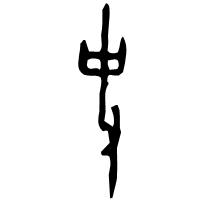
\includegraphics[width=\textwidth]{甲骨文/史}
		\caption{\content{史}{史}}
	\end{subcaptionblock}
	\begin{subcaptionblock}{.15\textwidth}
		\centering
		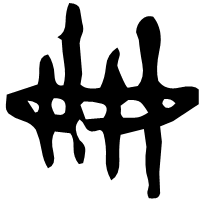
\includegraphics[width=\textwidth]{甲骨文/冊}
		\caption{\content{冊}{册}}
	\end{subcaptionblock}
	\begin{subcaptionblock}{.15\textwidth}
		\centering
		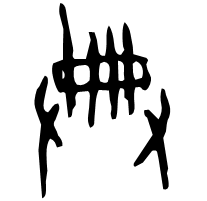
\includegraphics[width=\textwidth]{甲骨文/典}
		\caption{\content{典}{典}}
	\end{subcaptionblock}
	\caption{}
	\label{figure:甲骨文中的「史」「冊」「典」}
\end{wrapfigure}
\content{較近的考古證據則表明,商代人的主要書寫工具並不是甲骨,而是\textbf{毛筆和竹簡}。我們看\cref*{figure:甲骨文中的「史」「冊」「典」},甲骨文中「史」字描繪的是手拿筆桿寫字的模樣;「冊」字則像一排竹簡串起來的樣子;「典」字更形象,它描繪的是雙手端著竹簡的模樣。}{较近的考古证据则表明,商代人的主要书写工具不是甲骨,而是\textbf{毛笔和竹简}。我们看\cref*{figure:甲骨文中的「史」「冊」「典」},甲骨文中“史”字描绘的是手拿笔杆写字的模样;“册”字则像一排竹简串起来的样子;“典”字更形象,它描绘的是双手端着竹简的模样。}\par
\content{毛筆、竹簡要比龜甲、兽骨更易獲取,因此它的用途也就更「日常化」。但可惜的是,竹簡易腐,考古界至今也難以得到三千多年前的有字竹簡,所以罕有直接證據能夠說明當時竹簡的用途。}{毛笔、竹简要比龟甲、兽骨更易获取,因此它的用途也就更“日常化”。但可惜的是,竹简易腐,考古界至今也难以得到三千多年前的有字竹简,所以罕有直接证据能够说明当明当时竹简的用途。}\par
\content{而在同一時期,青銅器則要比甲骨更難獲取。因此青銅器上的\textbf{金文}就必須用來記錄最重要的事情,萬萬不能寫流水賬。就從出土文物來看,商代甲骨文多用於記錄祭祀、戰爭、狩猎、歷法、天象等,內容繁多;但商朝青銅器上的銘文就顯得惜字如金,大多只是記錄鑄者或其祖先的名稱,僅有廖廖幾字。}{而在同一时期,青铜器则要比甲骨更难获取。因此青铜器上的\textbf{金文}就必须用来记录最重要的事情,万万不能写流水账。就从出土文物来看,商代甲骨文多用于记录祭祀、战争、历法、天象等,内容繁多;但商朝青铜器上的铭文就显得惜字如金,大多只是记录铸者或其祖先的名称,仅有廖廖几字。}\par
\content{及至西周,乃至春秋、戰國,青銅器工藝漸臻成熟,產量也越來越高,人們對於金文的使用也不再那樣吝嗇。於是,舉凡王公貴族之事,無論大小,都可以記錄在青銅器上,金文的發展便在周代達到最盛;而殷商甲骨文則隨著商代的覆滅,一並失傳。}{及至西周,乃至春秋、战国,青铜器工艺渐臻成熟,产量也越来越高,人们对于金文的使用也不再那样吝啬。于是,举凡王公贵族之事,无论大小,都可以记录在青铜器上,金文的发展便在周代达到最盛;而殷商甲骨文则随着商代的覆灭,一并失传。}\par
\begin{wrapfigure}{O}{.4\textwidth}
	\centering
	\vspace{-1em}
	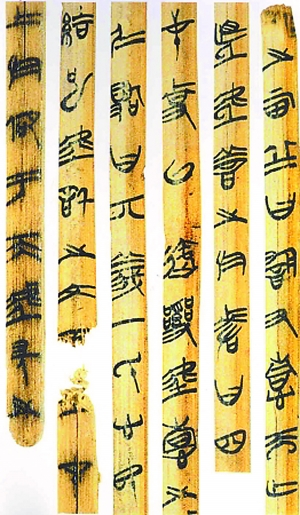
\includegraphics[width=.3\textwidth]{孔子詩論竹簡.jpg}
	\caption{\content{《孔子詩論》竹簡片段}{《孔子诗论》竹简片段}}
	\label{figure:《孔子詩論》竹簡片段}
\end{wrapfigure}
\content{春秋、戰國人也用竹簡寫字。\cref*{figure:《孔子詩論》竹簡片段}便是《孔子詩論》的竹簡書,其間所寫的文字應當是大篆的一種。除了竹簡之外,人們也偶爾使用\textbf{絲綢}(古稱「帛」)來書寫——這大概是中國歷史上最早的「紙」了。但絲綢既不像竹簡那樣廉價,又不像青銅器那樣容易保存,所以始終沒有普及開來。東漢蔡倫改進造紙術後,紙張的生產成本大大降低,這才逐漸取代笨重的竹簡,成為兩千多年來的主流書寫工具。}{春秋、战国人也用竹简写字。\cref*{figure:《孔子詩論》竹簡片段}便是《孔子诗论》的竹简书,其间所写的文字应当是大篆的一种。除了竹简之外,人们也偶尔使用\textbf{丝绸}(古称“帛”)来书写——这大概是中国历史上最早的“纸”了。但丝绸既不像竹简那样廉价,又不像青铜器那样容易保存,所以始终没有普及开来。东汉蔡伦改进造纸术后,纸张的生产成本大大降低,这才逐渐取代笨重的竹简,成为两千多年来的主流书写工具。}\par
\content{戰國時期雖有毛筆,但尚不成熟,很少被人使用。當時的人們在竹簡上寫字,通常是用竹簽點漆,或是用刀篆刻——這兩類書寫工具都算是「硬筆」。戰國末期的秦將蒙恬改進了毛筆,才使毛筆逐漸取代硬筆的地位,成為主流的書寫工具。}{战国时期虽有毛笔,但尚不成熟,很少被人使用。当时的人们在竹简上写字,通常是用竹签点漆,或是用刀篆刻——这两类书写工具都算是“硬笔”。战国末期的秦将蒙恬改进了毛笔,才使毛笔逐渐取代硬笔的地位,成为主流的书写工具。}\par
\content{毛筆和紙張對漢字演變有著重大意義。毛筆運筆靈活,細節豐富,變化無窮,書寫的多樣性比硬筆高出一個檔次,於是後世各種風格的楷書、行書、草書層出不窮。廉價的紙張對於文人墨客來說,同樣不可或缺。相傳王羲之每日練完書法都在住處附近的池中洗筆,經年累月竟把池水洗黑。若他是用絲綢練字的話,恐怕還沒練成就已傾家蕩產了。}{毛笔和纸张对汉字演变有着重大意义。毛笔运笔灵活,细节丰富,变化无穷,书写的多样性比硬笔高出一个档次,于是后世各种风格的楷书、行书、草书层出不穷。廉价的纸张对于文人墨客来说,同样不可或缺。相传王羲之每日练完书法都在住处附近的池中洗笔,经年累月竟把池水洗黑。若他是用丝绸写字的话,恐怕还没练成就已倾家荡产了。}\par
\content{到了現代,隨著硬筆生產技術的提高和人們對書寫效率的要求,硬筆又占據了主流市場;而紙張的地位則從未被撼動。不過現代人還多了一套「書寫工具」,那就是——鍵盤、熒屏和印表機。}{到了现代,随着硬笔生产技术的提高和人们对书写效率的要求,硬笔又占据了主流市场;而纸张的地位则从未被撼动。不过现代人还多了一套“书写工具”,那就是——键盘、屏幕和打印机。}\par
\subsection{\content{印刷術的發展}{印刷术的发展}}\label{subsection:印刷術的發展}
\begin{boxquote}{\content{《農書·麻苧門》}{《农书·麻苎门》}}
	\content{後世有人別生巧技,以鐵為印盔,界行內用稀瀝青澆滿,冷定取平。火上再行煨化,以燒熟瓦字,排于行內,作活字印板。}{后世有人别生巧技,以铁为印盔,界行内用稀沥青浇满,冷定取平。火上再行煨化,以烧熟瓦字,排于行内,作活字印板。}
\end{boxquote}
\content{印刷與手寫大不相同。我們談書法中的「字體」,最常講的是「楷書」「行書」「草書」這些概念;但談及電腦字體和印刷字體,最常講的卻是「明體(宋體)」「楷體」「黑體」「仿宋體」這些概念。本小節我們只聚焦於印刷;至於電腦漢字,我將單獨撰寫一節內容來介紹它。}{印刷与手写大不相同。我们谈书法中的“字体”,最常讲的是“楷书”“行书”“草书”这些概念;但谈及电脑字体和印刷字体,最常讲的却是“宋体(明体)”“楷体”“黑体”“仿宋体”这些概念。本小节我们只聚焦于印刷;至于电脑汉字,我将单独撰写一节内容来介绍它。}\par
\content{最早的印刷工具當屬\textbf{印章}。古人用刀具將文字反刻在銅塊、銀塊、玉塊等材料上,然後就可以用它蘸取印泥(通常是紅色的),印下油墨,這就是一種「印刷」了。}{最早的印刷工具当属\textbf{印章}。古人用刀具将文字反刻在铜块、银块、玉块等材料上,然后就可以用它蘸取印泥(通常是红色的),印下油墨,这就是一种“印刷”了。}\par
\begin{wrapfigure}{O}{.51\textwidth}
	\centering
	\begin{subcaptionblock}{.25\textwidth}
		\centering
		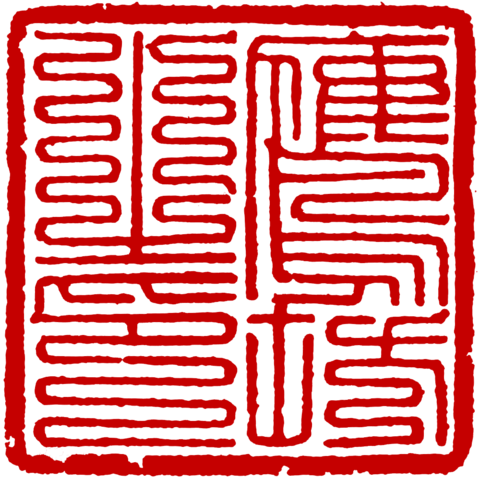
\includegraphics[width=\textwidth]{九疊篆印章「鷹坊之印」.png}
		\caption{\content{九疊篆陽文印}{九叠篆阳文印}}
		\label{figure:九疊篆陽文印「鷹坊之印」}
		\footnotesize{\color{darkgray}\content{「鷹坊之印」}{“鹰坊之印”}}
	\end{subcaptionblock}
	\begin{subcaptionblock}{.25\textwidth}
		\centering
		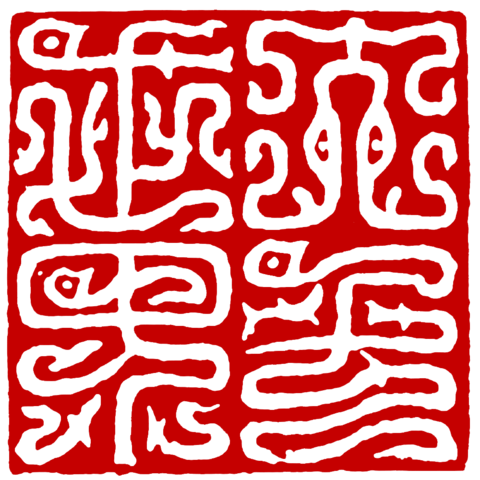
\includegraphics[width=\textwidth]{鳥蟲篆印章「大千世界」.png}
		\caption{\content{鳥蟲篆陰文印}{鸟虫篆阴文印}}
		\label{figure:鳥蟲篆陰文印「大千世界」}
		\footnotesize{\color{darkgray}\content{「大千世界」}{“大千世界”}}
	\end{subcaptionblock}
	\caption{}
	\vspace{-1em}
\end{wrapfigure}
\content{根據印文的凹凸,我們可以把印章分為「陽文印」和「陰文印」。陽文印是文字部分凸起,所以印出來得到的是白底紅字(\cref*{figure:九疊篆陽文印「鷹坊之印」});陰文印是文字部分凹下,所以印出來得到的是紅底白字(\cref*{figure:鳥蟲篆陰文印「大千世界」})。}{根据印文的凹凸,我们可以把印章分为“阳文印”和“阴文印”。阳文印是文字部分凸起,所以印出来得到的是白底红字(\cref*{figure:九疊篆陽文印「鷹坊之印」});阴文印是文字部分凹下,所以印出来得到的是红底白字(\cref*{figure:鳥蟲篆陰文印「大千世界」})。}\par
\content{印章從春秋戰國時期就開始流行了。當時的主要文字是大篆,所以印章普遍使用篆文刻成。後世也往往使用篆文,而很少有使用楷書、行書、草書來刻章的——可能是文人尚古的風氣使然,也可能是篆文顯得嚴肅、莊重。但筆者認為還有一個關鍵因素:用刀這樣的硬筆來刻寫毛筆字,實在是不容易。}{印章从春秋战国时期就开始流行了。当时的主要文字是大篆,所以印章普遍使用篆文刻成。后世也往往使用篆文,而很少有使用楷书、行书、草书来刻章的——可能是文人尚古的风气使然,也可能是篆文显得严肃、庄重。但笔者认为还有一个关键因素:用刀这样的硬笔来刻写毛笔字,实在是不容易。}\par
\content{\textbf{雕版印刷}則是真正意義上的「印刷術」。隋唐時期,人們先用毛筆把文字寫在特別薄的宣紙上,然後把紙張反貼在木板上,再由雕刻師傅挖掉沒有墨跡的地方,這樣就造好了一塊「印版」。印刷時,只需在印版上刷好墨,再鋪紙按壓,即可完成一次印刷。所以在這一時期,印刷品上所印的自然是楷書。}{\textbf{雕版印刷}则是真正意义上的“印刷术”。隋唐时期,人们先用毛笔把文字写在特别薄的宣纸上,然后把纸张反贴在木板上,再由雕刻师傅挖掉没有墨迹的地方,这样就造好了一块“印版”。印刷时,只需要印版上刷好墨,再铺纸按压,即可完成一次印刷。所以在这一时期,印刷品上所印的自然是楷书。}\par
\content{宋朝及以後,印刷業空前繁榮,書籍、紙鈔等印刷品開始普及到庶民階層。為了應對爆發式增長的印刷需求,印刷業也急需改進原本的工藝和流程。刻字工們不再照著宣紙上的墨跡刻版了,而是乾脆徒手刻字,以求速成。}{宋朝及以后,印刷业空前繁荣,书籍、纸钞等印刷品开始普及到庶民阶层。为了应对爆发式增长的印刷需求,印刷业也急需改进原本的工艺和流程。刻字工们不再照着纸上的墨迹刻版了,而是干脆徒手刻字,以求速成。}\par
\content{但徒手刻字還面臨一個很大的問題:要用\cref*{figure:徒手刻版}那樣的硬筆還原出毛筆的細節,實在是費時費力,事倍功半。所以從宋朝開始,刻字工們逐漸改變了楷書的筆畫,化曲為直,務求易於刻制。到明朝初年,印刷界已經產生了一種較為成熟的字體——\textbf{明體(也稱宋體)}。這是印刷字體與書法字體分道揚鑣的開始。}{但徒手刻字还面临一个很大的问题:要用\cref*{figure:徒手刻版}那样的硬笔还原出毛笔的细节,实在是费时费力,事倍功半。所以从宋朝开始,刻字工们逐渐改变了楷书的笔画,化曲为直,务求易于刻制。到明朝初年,印刷界已经产生了一种较为成熟的字体——\textbf{宋体(也称明体)}。这是印刷字体与书法字体分道扬镳的开始。}\par
\begin{figure}[H]
	\centering
	\begin{tikzpicture}
		\definecolor{seal red}{HTML}{C50000}
		\node[inner sep=0pt](main)at(-.78,0){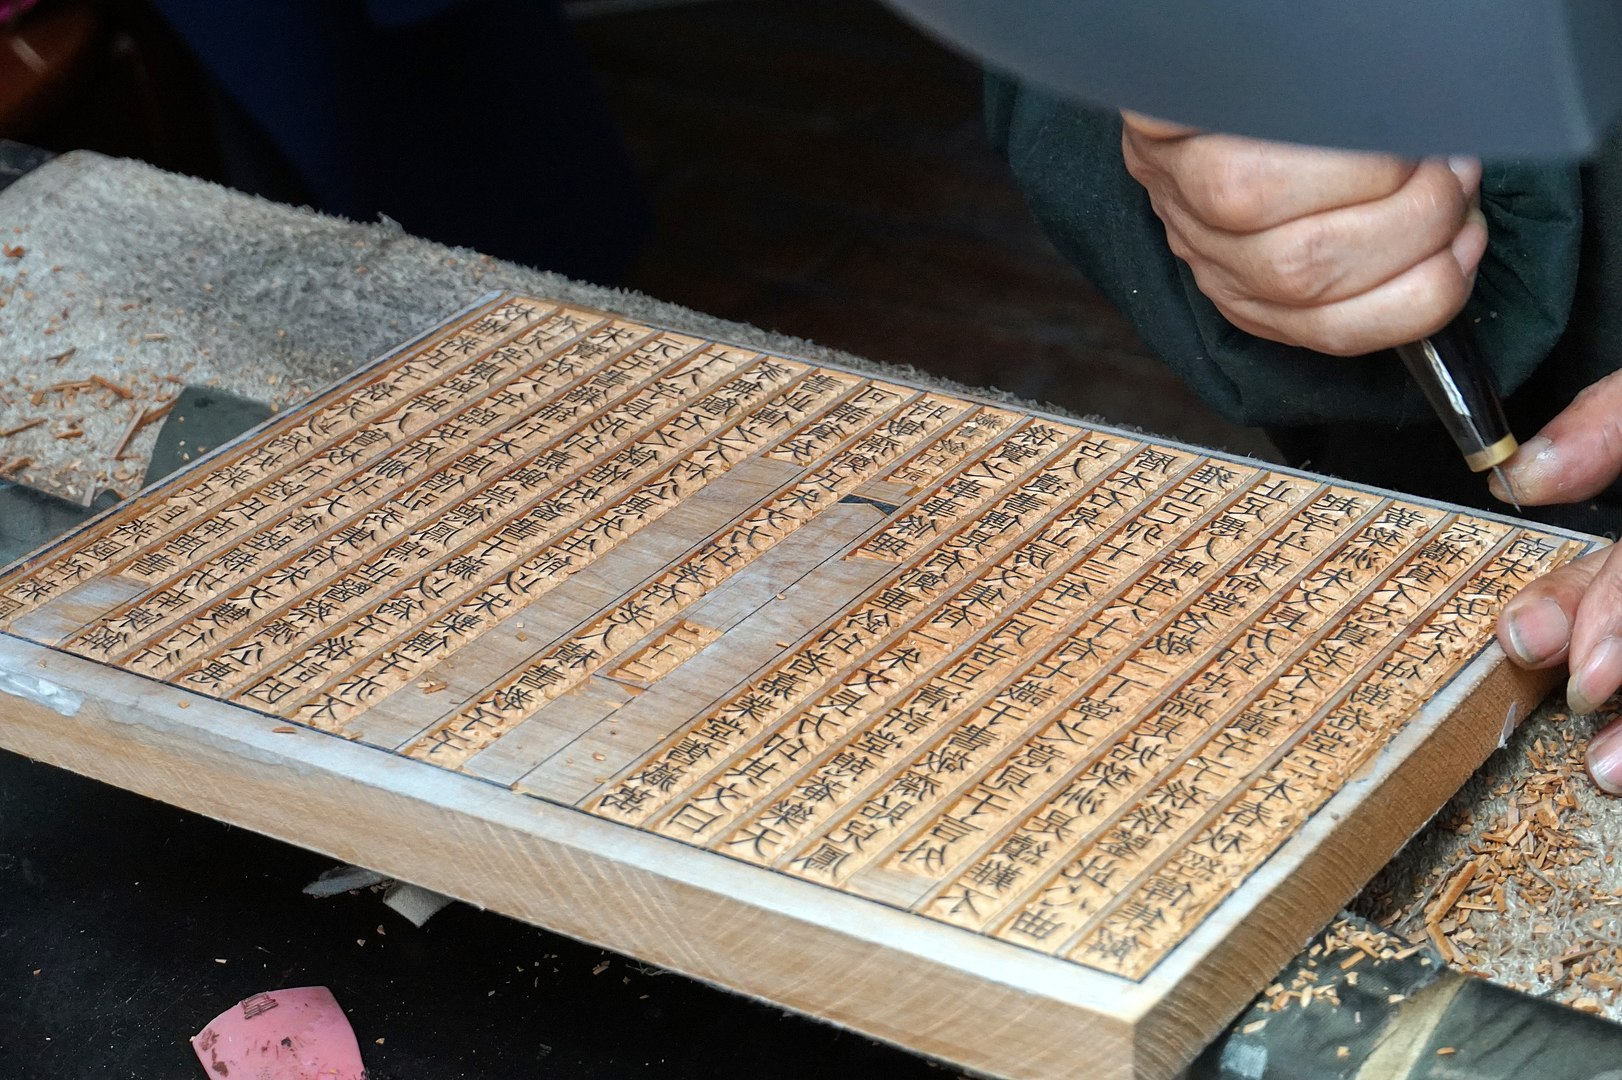
\includegraphics[width=.5\textwidth]{徒手刻版.jpg}};
		\begin{scope}
			\clip(8,0)circle(2.5);
			\node[inner sep=0pt]at(-8.4,-1.6){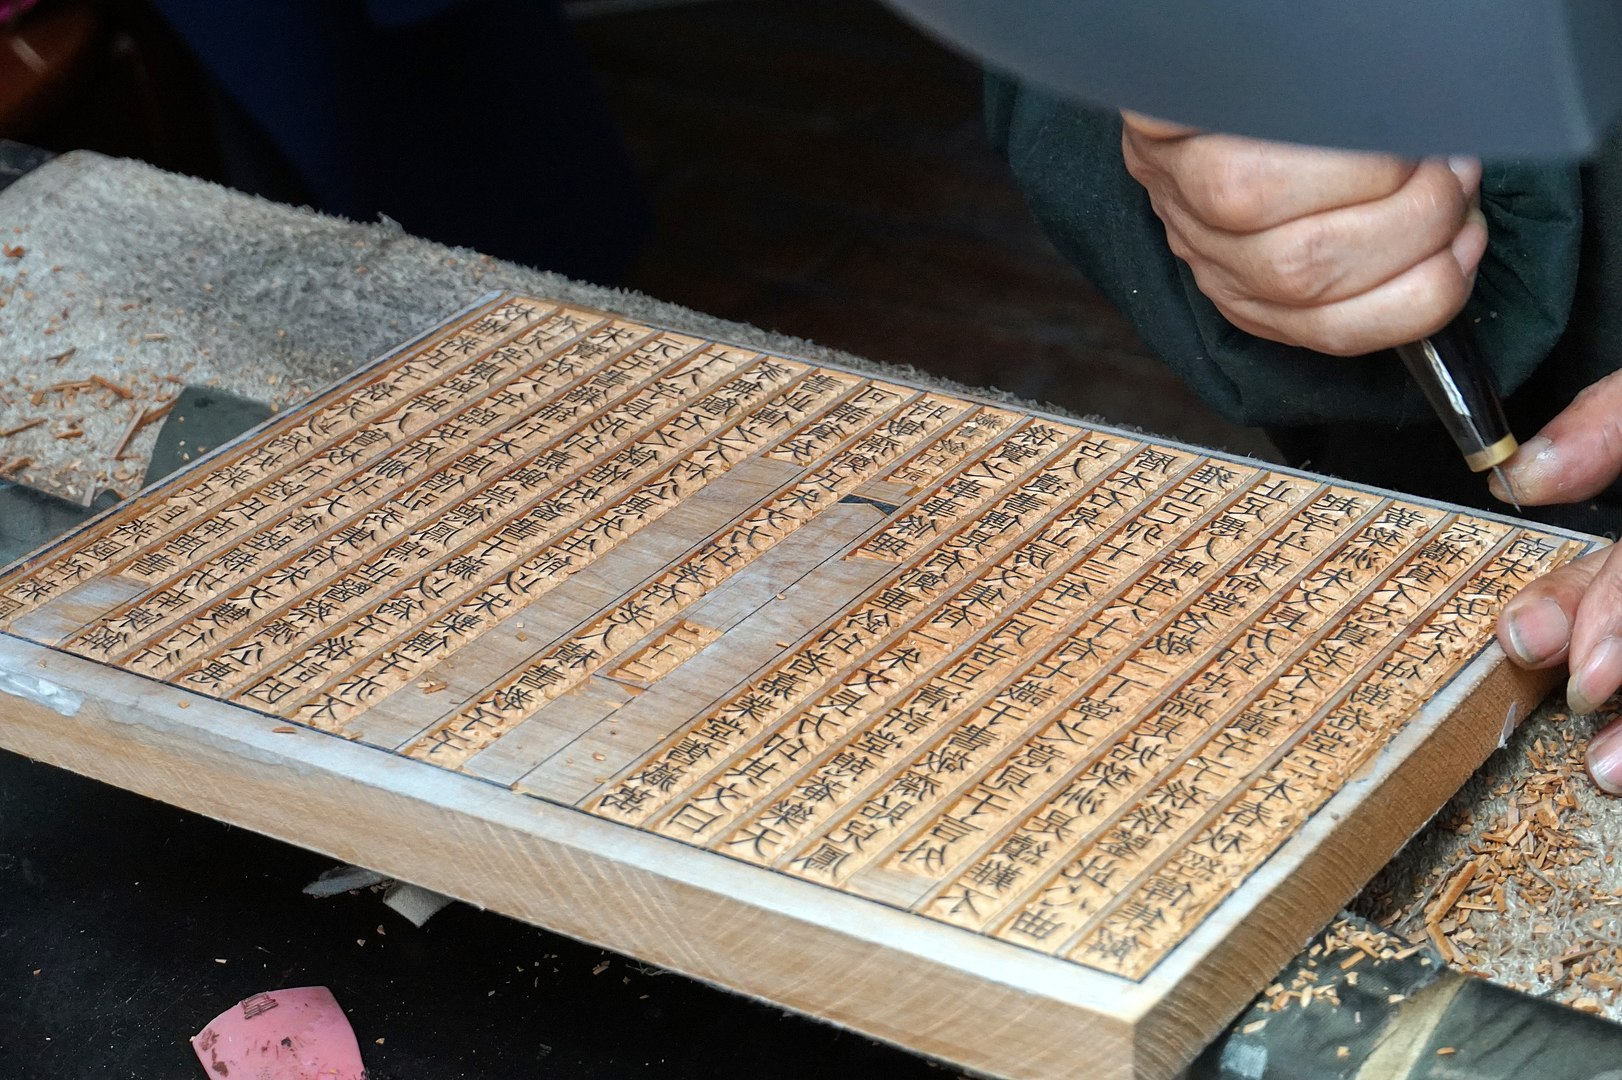
\includegraphics[width=2.5\textwidth]{徒手刻版.jpg}};
		\end{scope}
		\node[draw,circle,seal red,thin,minimum size=1cm](small)at(2.5,.32){};
		\node[draw,circle,seal red,minimum size=5cm](big)at(8,0){};
		\draw[dashed,seal red](tangent cs:node=small,point={(big.south)},solution=2)--(tangent cs:node=big,point={(small.south)},solution=1);
		\draw[dashed,seal red](tangent cs:node=small,point={(big.north)},solution=1)--(tangent cs:node=big,point={(small.north)},solution=2);
	\end{tikzpicture}
	\caption{\content{徒手刻版}{徒手刻版}}
	\label{figure:徒手刻版}
\end{figure}
\content{北宋的畢昇發明了\textbf{活字印刷術}。這種方法不再是以版面為單位來印刷,而是以漢字為單位來印刷。刻字工只需要預先刻好所需文字,把它們做成字模(稱為「活字」),就可以任意取用。於是,昨天用來印《水滸傳》的字,明天還能取下來印《紅樓夢》,而不需要另外刻版,這是何等方便的事!}{北宋的毕昇发明了\textbf{活字印刷术}。这种方法不再是以版面为单位来印刷,而是以汉字为单位来印刷。刻字工只需要预先刻好所需文字,把它们做成字模(称为“活字”),就可以任意取用。于是,昨天用来印《水浒传》的字,明天还能取下来印《红楼梦》,而不需要另外刻版,这是何等方便的事!}\par
\content{但活字印刷也有一些缺點,這使得它在古代的中國並不如雕版印刷那樣流行。比如說,活字印刷只能刻印文字,而雕版印刷既可以刻印文字,又可以刻印圖像。那麼,若是要印全本繡像《金瓶梅》的話,活字印刷就顯得有些捉襟見肘了。}{但活字印刷也有一些缺点,这使得它在古代的中国并不如雕版印刷那样流行。比如说,活字印刷只能刻印文字,而雕版印刷既可以刻印文字,又可以刻印图像。那么,若是要印全本绣像《金瓶梅》的话,活字印刷就显得有些捉襟见肘了。}\par
\content{更致命的問題是,漢字數量繁多,活字印刷前需要預先投入巨大的工作量,才能準備好充足的活字\footnote{而且很多常用字可能在同一版面出現幾次甚至十幾次,所以需要有多個備用字,這又是很大的工作量。}。但歐文只有幾十個字母,制作活字的工作量要小很多,因此活字印刷術才能在歐洲大放異彩,從而推動了歐洲印刷的工業化進程。}{更致命的问题是,汉字数量繁多,活字印刷前需要预先投入巨大的工作量,才能准备好充足的活字\footnote{而且很多常用字可能在同一版面出现几次甚至十几次,所以需要有多个备用字,这又是很大的工作量。}。但欧文只有几十个字母,制作活字的工作量要小很多,因此活字印刷术才能在欧洲大放异彩,从而推动了欧洲的工业化进程。}\par
\content{現代印刷術已經不以「字」為單位了——甚至說,根本不需要「字」這個概念。印表機的眼中只有數以億計的密密麻麻的點,而它要做的就是在正確的點位加上正確的墨。於是,無論文字、圖畫、數學式,還是什麼奇奇怪怪的符號,印表機都可以在幾秒之內搞定,就像魔術一樣。}{现代印刷术已经不以“字”为单位了——甚至说,本不需要“字”这个概念。打印机的眼中只有数以亿计的密密麻麻的点,而它要做的就是在正确的点位加上正确的墨。于是,无论文字、图画、数学式,还是什么奇奇怪怪的符号,打印机都可以在几秒之内搞定,就像魔术一样。}\par
\content{電腦和印表機的出現打破了硬筆的局限,使人類對字體細節的控制能力提高到了前所未有的水平。短短幾十年間,中文印刷界就出現了各種各樣不同的黑體、圓體、仿宋體,以及富有特色的綜藝體、疊圓體等——當然還有在台灣風靡一時的康熙字典體。}{电脑和打印机的出现打破了硬笔的局限,使人类对字体细节的控制能力提高到了前所未有的水平。短短几十年间,中文印刷界就出现了各种各样不同的黑体、圆体、仿宋体,以及富有特色的综艺体、叠圆体等——当然还有在台湾风靡一时的康熙字典体。}\par
\content{按唐䦨先生的說法\footnote{見《中國文字學》第二十節「繪畫·鍥刻·書寫·印刷」。},印刷術對字體的「穩定」也有貢獻。在沒有印刷術的時候,人們要想複製經典,只能手寫傳抄。不同人的字跡不盡相同,反覆傳抄之下難免產生許多新的寫法;傳抄過程中也有可能出現錯誤,所以不同版本的書在可能同一句話的個別字上有幾種不同的說法。印刷術一舉改變了這兩種情況,既統一了內容,又統一了字體。}{按唐兰先生的说法\footnote{见《中国文字学》第二十节“绘画·锲刻·书写·印刷”。},印刷术对字体的“稳定”也有贡献。在没有印刷术的时候,人们要想复制经典,只能手写传抄。不同人的字迹不尽相同,反复传抄之下难免产生许多新的写法;传抄过程中也有可能出现错误,所以不同版本的书可能在同一句话的个别字上有几种不同的说法。印刷术一举改变了这两种情况,既统一了内容,又统一了字体。}\par
\subsection{\content{漢朝的文字與文字研究}{汉朝的文字与文字研究}}\label{subsection:漢朝的文字與文字研究}
\begin{wrapfigure}{O}{8.6cm}
	\centering
	\vspace{-2ex}
	\begin{boxhorizontalcompare}[width=8.6cm,lefthand width=4.2cm]
		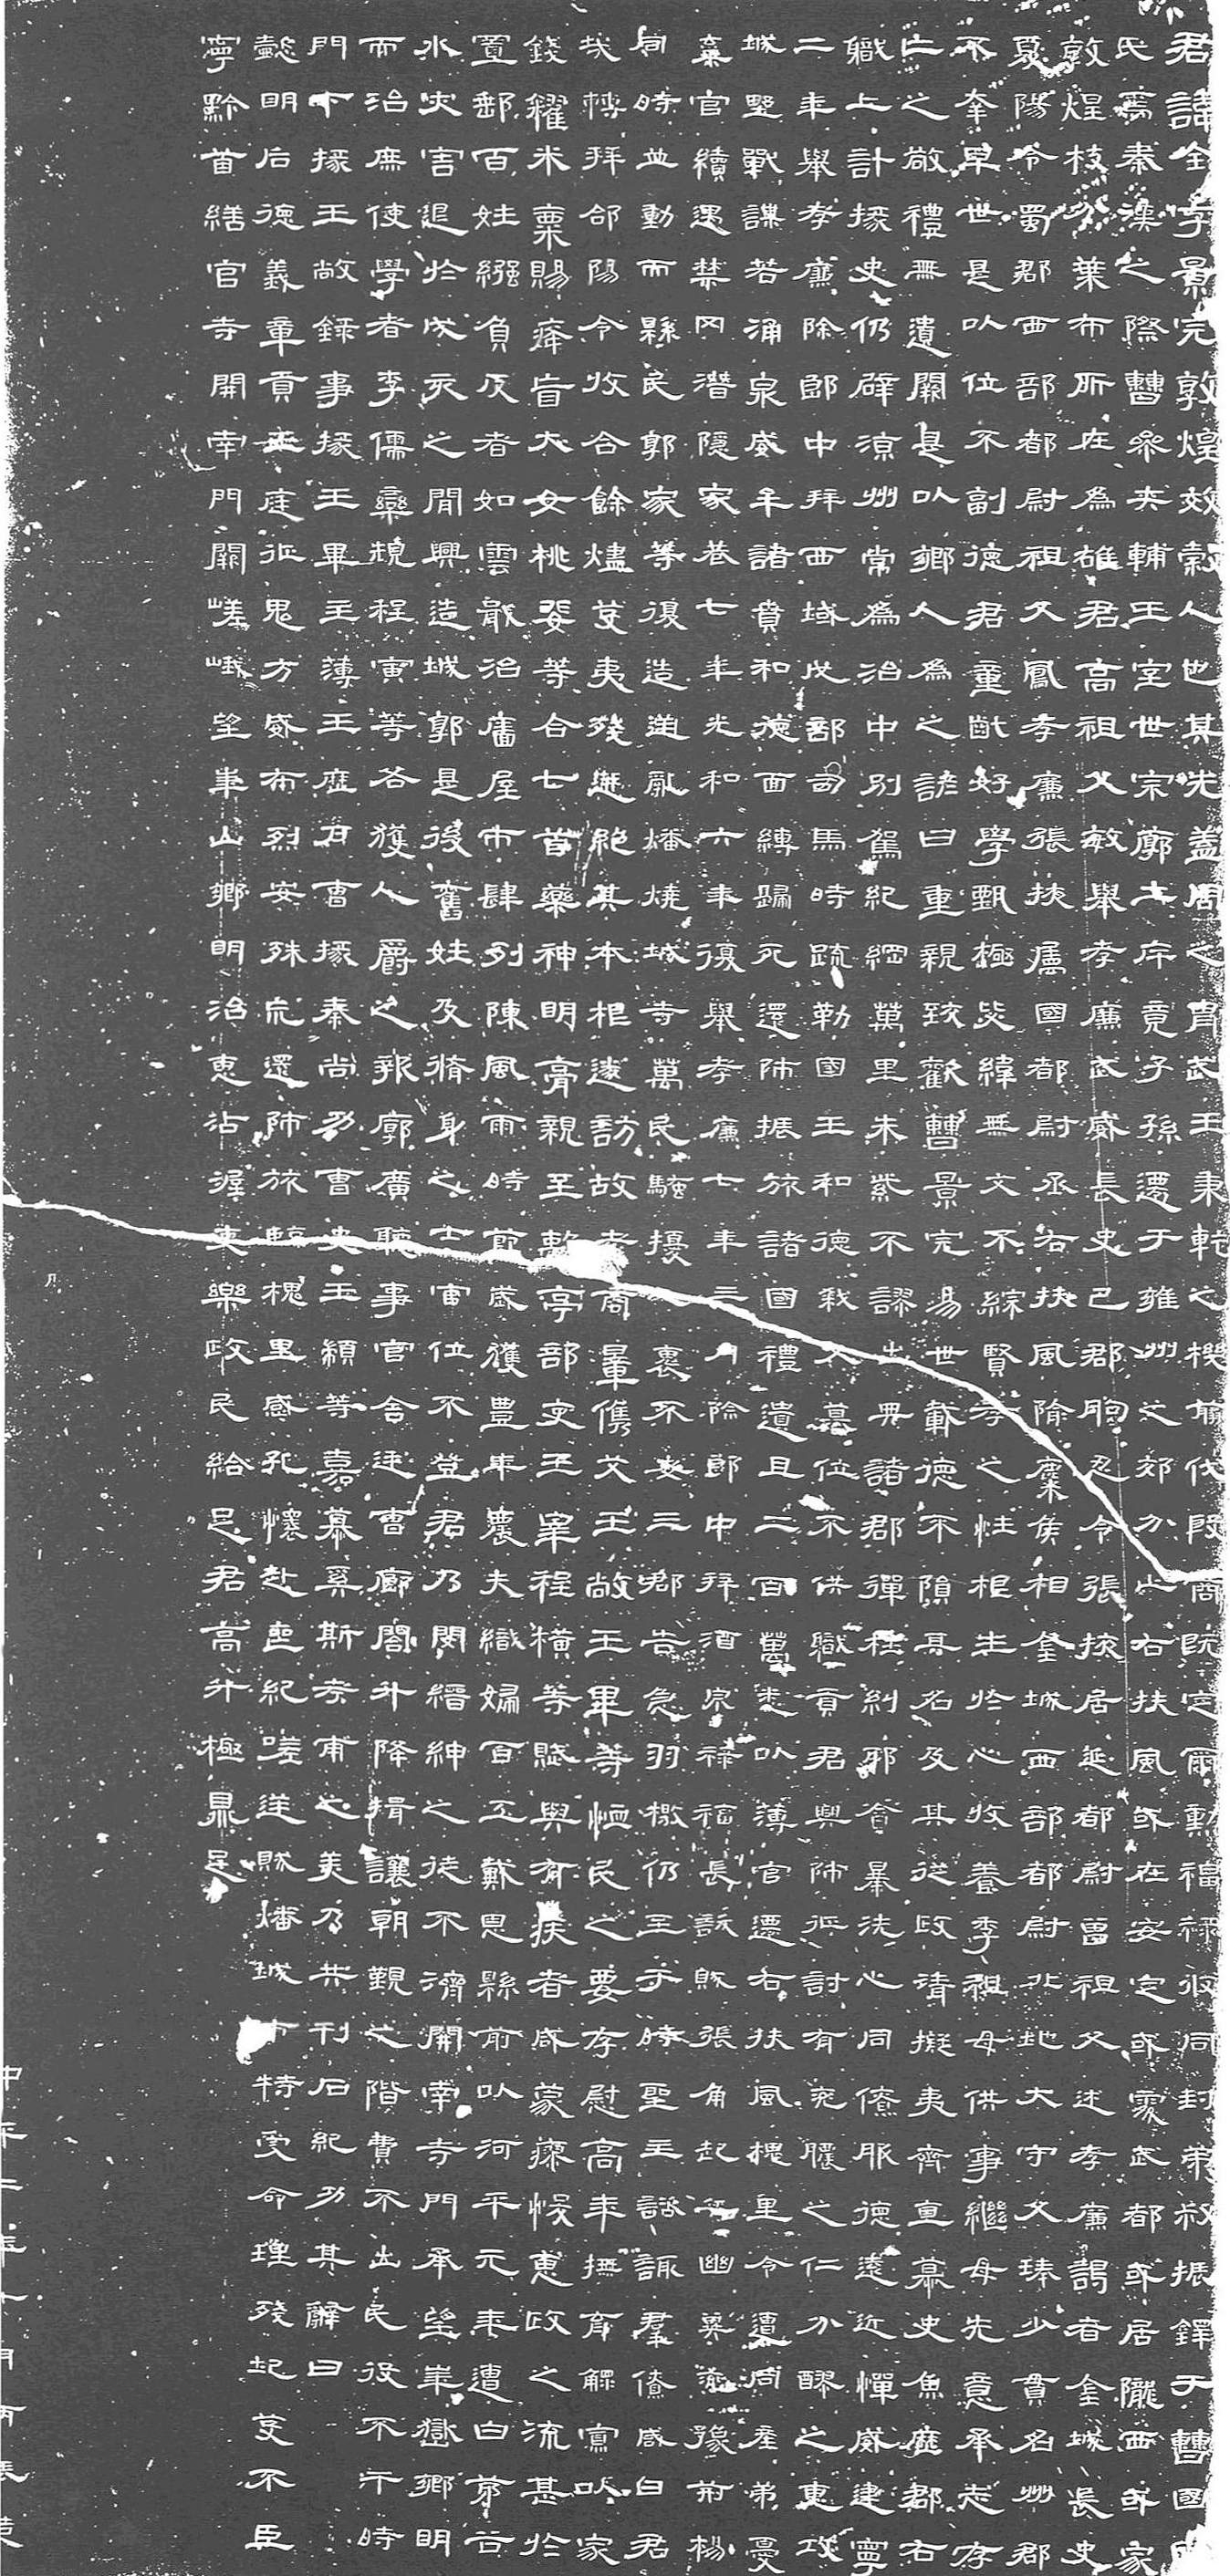
\includegraphics[scale=.32,trim={930pt 1950pt 10pt 25pt},clip]{曹全碑.jpg}
	\tcblower
		\color{white}\hspace{-6.45mm}\vspace{-1.2mm}
		\begin{NiceTabular}[cell-space-limits=4.1pt]{*{7}{W{c}{.1cm}}}
			職 & 亡 & 不 & 夏 & 敦 & 氏 & 君 \\
			上 & 之 & 幸 & 陽 & 煌 & 焉 & 諱 \\
			計 & 敬 & 早 & 令 & 枝 & 秦 & 全 \\
			掾 & 禮 & 世 & 蜀 & 分 & 漢 & 字 \\
			史 & 無 & 是 & 郡 & 葉 & 之 & 景 \\
			仍 & 遺 & 以 & 西 & 布 & 際 & 完 \\
			辟 & 闕 & 位 & 部 & 所 & 曹 & 敦 \\
			涼 & 是 & 不 & 都 & 在 & 參 & 煌 \\
			州 & 以 & 副 & 尉 & 爲 & 夾 & 效 \\
			常 & 鄉 & 德 & 祖 & 雄 & 輔 & 穀 \\
			爲 & 人 & 君 & 父 & 君 & 王 & 人 \\
			治 & 爲 & 童 & 鳳 & 高 & 室 & 也 \\
			中 & 之 & 齔 & 孝 & 祖 & 世 & 其 \\
			別 & 諺 & 好 & 廉 & 父 & 宗 & 先 \\
		\end{NiceTabular}
	\end{boxhorizontalcompare}
	\caption{\content{〈曹全碑〉片段}{《曹全碑》片段}}
	\footnotesize{\color{darkgray}\content{左為隸書碑文,右為正體字釋文}{左为隶书碑文,右为繁体字释文}}
	\label{figure:《曹全碑》片段}
\end{wrapfigure}
\content{兩漢時期對於漢字來說,是一個重要的歷史階段。一方面,漢字的形態漸臻成熟,其後直到近代,都不再有劇烈的字形變化了;另一方面,漢朝人開始了對古文字的系統性研究,形成了新的理論,這也是前人未有之成果。}{两汉时期对于汉字来说,是一个重要的历史阶段。一方面,汉字的形态渐臻成熟,其后直到近代,都不再有剧烈的字形变化了;另一方面,汉朝人开始了对古文字的系统性研究,形成了新的理论,这也是前人未有之成果。}\par
\content{今天人們所用的大部分正體字,其實早在漢朝就已基本定型了。以東漢〈曹全碑〉為例,它是用隸書寫成的。現代人不必專門研習古文字,就可以看懂其中的絕大部分字(\cref*{figure:《曹全碑》片段})。換言之,隸書正是古今文字的分水嶺。}{汉字形态发生剧烈变化的时期,主要在殷商到秦汉之间。今天人们所用的大部分繁体字,其实早在汉朝就已基本定型了。以东汉《曹全碑》为例,它是用隶书写成的。现代人不必专门研习古文字,只要能看懂繁体字,就能看懂碑上的绝大部分字(\cref*{figure:《曹全碑》片段})。换言之,隸書正是古今文字的分水嶺。}\par
\content{今天我們熟知的楷書、行書、草書,它們的早期形態也全都出現在漢朝。所以我們說漢朝是承前啟後的時代,這樣的說法毫不誇張。}{今天我们熟知的楷书、行书、草书,它们的早期形态也全都出现在汉朝。所以我们说汉朝是一个承前启后的时代,这样的说法毫不夸张。}\par
\subsubsection*{\content{漢人眼中的「古文」}{汉人眼中的“古文”}}
\begin{boxquote}{\content{《說文解字·序》}{《说文·序》}}
	\content{其後諸侯力政,不統於王。惡禮樂之害己,而皆去其典籍。分為七國,田疇異畝,車涂異軌,律令異法,衣冠異制,言語異聲,文字異形。秦始皇帝初兼天下,丞相李斯乃奏同之,罷其不與秦文合者。}{其后诸侯力政,不统于王。恶礼乐之害己,而皆去其典籍。分为七国,田畴异亩,车涂异轨,律令异法,衣冠异制,言语异声,文字异形。秦始皇帝初兼天下,丞相李斯乃奏同之,罢其不与秦文合者。}
\end{boxquote}
\content{戰國時期的各國文字本來同源於西周金文,但由於地理隔閡、政治割據等原因,同樣的文字在不同地區可能演變出不同的形態\footnote{一般可以將戰國文字分為五系文字:秦文字、楚文字、三晉文字、齊文字、燕文字。三晉文字並不見得完全統一,但差異較小。}。秦滅六國後,李斯提議統一文字,於是整理出「小篆」;後來又提議焚書,遂有「挾書律」\footnote{挾書律相當嚴苛,對私自收藏持有違禁書籍的人處以滅族。該律令在前213年頒布,漢初仍然施行,直到前191年廢除,跨了一代人的時間。}。慢慢地,山東六國的文字就逐漸失傳了,只有秦系文字這一脈得到保留,即:西周春秋金文——戰國秦系文字——秦朝小篆——汉朝隸書。}{战国时期的各国文字本来同源于西周金文,但由于地理隔阂、政治割据等原因,同样的文字在不同地区可能演变出不同的形态\footnote{一般可以将战国文字分为五系文字:秦文字、楚文字、三晋文字、齐文字、燕文字。三晋文字并不见得完全统一,但差异较小。}。秦灭六国后,李斯提议统一文字,于是整理出“小篆”;后来又提议焚书,遂有“挟书律”\footnote{挟书律相当严苛,对私自收藏持有违禁书籍的人处以灭族。该律令在前213年颁布,汉初仍然施行,直到前191年废除,跨了一代人的时间。}。慢慢地,山东六国的文字就逐渐失传了,只有秦系文字这一脉得到保留,即:西周春秋金文——战国秦系文字——秦朝小篆——汉朝隶书。}\par
\content{西漢初年,有不少學者根據自己的記憶,還原出了六國經書的內容——這些版本的經書自然是用當時通行的隸書來書寫的,稱為\textbf{今文經};等到挾書律廢除,民間私藏的書籍也慢慢浮現出來——這些版本的經書自然是用六國文字來書寫的,稱為\textbf{古文經}。不同學者解釋經文的理念不同,由此引發分歧,最後形成了兩個學派:今文經學派和古文經學派。}{西汉初年,有不少学者根据自己的记忆,还原出了六国经书的内容——这些版本的经书自然是用当时通行的隶书来书写的,称为\textbf{今文经};等到挟书律废除,民间私藏的书籍也慢慢浮现出来——这些版本的经书自然是用六国文字来书写的,称为\textbf{古文经}。不同学者解释经文的理念不同,由此引发分歧,最后形成了两个学派:今文经学派和古文经学派。}\par
\content{古文經學派的興起相當晚\footnote{按裘錫圭的說法,是到西漢末期才正式形成。},彼時人們早已不知道六國文字了。當時的人們發現這些文字和最古老的籀文\footnote{漢人不知甲骨文,認為西周宣王時代的籀文就是有記載的最早的文字了。今人在籀文的所處時代方面有激烈的爭論,但漢人並未懷疑。}相比還有不少出入,便誤以為這是更古老的文字,所以叫它「古文」。今人已經知道「古文」實際是六國文字,其實並沒有那麼「古」。}{古文经学派的兴起相当晚\footnote{按裘锡圭的说法,是到西汉末期才正式形成。},彼时人们早已不知道六国文字了。当时的人们发现这些文字和最古老的籀文\footnote{汉人不知甲骨文,认为西周宣王时代的籀文就是有记载的最早的文字了。今人在籀文的所处时代方面有激烈的争论,但汉人并未怀疑。}相比还有不少出入,便误以为这是更古老的文字,所以叫它“古文”。今人已经知道“古文”实际是六国文字,其实并没有那么“古”。}\par
\subsubsection{\content{古字形的重要性}{古字形的重要性}}
\content{漢語博大精深,由此帶來的一個副作用便是,我們在解釋很多文字時,即便信口胡說,也能講出幾分道理來。王安石(王荊公)曾撰《字說》解釋文字,並利用自己的政治手腕大肆宣揚。如今此書已經失傳,但仍有不少笑話得以流傳下來:}{汉语博大精深,由此带来的一个副作用便是,我们在解释很多文字时,即便信口胡说,也能讲出几分道理来。王安石(王荆公)曾撰《字说》解释文字,并利用自己的政治手腕大肆宣扬。如今此书已经失传,但仍有不少笑话得以流传下来:}\par
\begin{boxquote}{\content{《邵氏聞見後錄·卷二十》}{《邵氏闻见后录·卷二十》}}
	\content{王荊公晚喜說字。客曰:覇字何以從西?荊公以西在方域主殺伐,累言數百不休。或曰:霸從雨,不從西也。荊公隨輒曰:如時雨化之耳。其學務鑿,無定論類此。}{王荆公晚喜说字。客曰:覇字何以从西?荆公以西在方域主杀伐,累言数百不休。或曰:霸从雨,不从西也。荆公随辄曰:如时雨化之耳。其学务凿,无定论类此。}
\end{boxquote}
\begin{boxquote}{\content{〈調謔編〉}{《调谑编》}}
	\content{東坡嘗舉「坡」字問荊公何義,公曰:「坡者土之皮。」東坡曰:「然則滑者水之骨乎?」荊公默然。}{东坡尝举“坡”字问荆公何义,公曰:“坡者土之皮。”东坡曰:“然则滑者水之骨乎?”荆公默然。}
\end{boxquote}
\content{大概王安石一時間沒有想到怎麼解釋「滑」字為妙,因而默然。否則他就會像解釋「霸」字那樣,找個似是而非的說法圓回來。}{大概王安石一时间没有想到怎么解释“滑”字为妙,因而默然。否则他就会像解释“霸”字那样,找个似是而非的说法圆回来。}\par
\content{從王安石的思路來看,他應該是用當時的正體(楷書)字形來解釋文字的。但是他或許沒有想到,兩千年來漢字的字形和字義都在不斷變化,其間發生了無數的分化、合併、改造、假借,乃至訛傳,即便用古字形來解釋,尚有許多說不清的地方,遑論楷書字形?筆者記得小學時國文老師講,身體部位和器官,如「肝膽股肱胃腎」之類,大多用「月」作偏旁。可惜今人無從知道王荊公對此有何高見了。}{从王安石的思路来看,他应该是用当时的正体(楷书)字形来解释文字的。但是他或许没有想到,两千年来汉字的字形和字义都在不断变化,其间发生了无数的分化、合并、改造、假借,乃至讹传,即便用古字形来解释,尚有许多说不清的地方,遑论楷书字形?笔者记得小学时语文老师讲,身体部位和器官,如“肝胆股肱胃肾”之类,大多用“月”作偏旁。可惜今人无从知道王荆公对此有何高见了。}\par
\content{其實以上六字的「月」旁都是「肉」旁。我們看\cref*{figure:《說文》小篆中的「月」與「肉」}《說文》小篆\footnote{「肱」原作「厷」,至西周晚期尚寫作\includecharacter{金文/肱},其偏旁顯然是後加的;另五字不見於甲骨文。故以《說文》小篆作為參考。}的字形,「月」與「肉」極為相像,以致我們很難認清這六字的偏旁究竟為何。等到楷書之後,作為獨體字的「肉」已從形狀上與「月」分開,但作為偏旁的「肉」則已經與「月」合流了。身體部位和器官以「肉」作偏旁當然合理;如果非抓著楷書「月」旁一定要扯到月亮上去,那豈不是誤人子弟!}{其实以上六字的“月”旁都是“肉”旁。我们看\cref*{figure:《說文》小篆中的「月」與「肉」}《说文》小篆\footnote{“肱”原作“厷”,至西周晚期尚写作\includecharacter{金文/肱},其偏旁显然是后加的;另五字不见于甲骨文。故以《说文》小篆作为参考。}的字形,“月”与“肉”极为相像,以致我们很难认清这六字的偏旁究竟为何。等到楷书之后,作为独体字的“肉”已从形状上与“月”分开,但作为偏旁的“肉”则已经与“月”合流了。身体部位和器官以“肉”作偏旁当然合理;如果非抓着楷书“月”旁一定要扯到月亮上去,那岂不是误人子弟!}\par
\begin{figure}[H]
	\centering
	\begin{subcaptionblock}{.1\textwidth}
		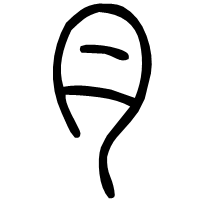
\includegraphics[width=\textwidth]{小篆/月}
		\caption*{月}
	\end{subcaptionblock}
	\begin{subcaptionblock}{.1\textwidth}
		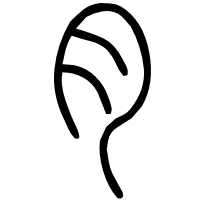
\includegraphics[width=\textwidth]{小篆/肉}
		\caption*{肉}
	\end{subcaptionblock}
	\begin{subcaptionblock}{.1\textwidth}
		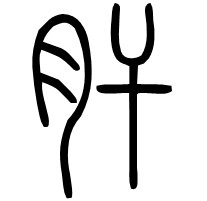
\includegraphics[width=\textwidth]{小篆/肝}
		\caption*{肝}
	\end{subcaptionblock}
	\begin{subcaptionblock}{.1\textwidth}
		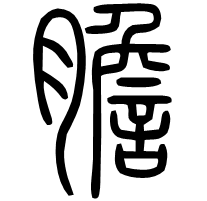
\includegraphics[width=\textwidth]{小篆/膽}
		\caption*{\content{膽}{膽(胆)}}
	\end{subcaptionblock}
	\begin{subcaptionblock}{.1\textwidth}
		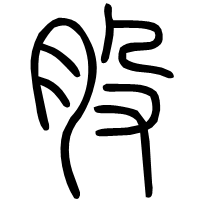
\includegraphics[width=\textwidth]{小篆/股}
		\caption*{股}
	\end{subcaptionblock}
	\begin{subcaptionblock}{.1\textwidth}
		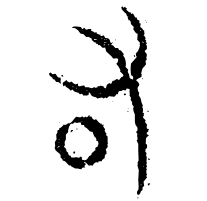
\includegraphics[width=\textwidth]{小篆/肱}
		\caption*{肱}
	\end{subcaptionblock}
	\begin{subcaptionblock}{.1\textwidth}
		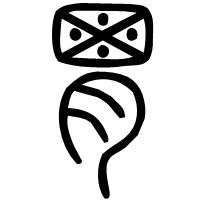
\includegraphics[width=\textwidth]{小篆/胃}
		\caption*{胃}
	\end{subcaptionblock}
	\begin{subcaptionblock}{.1\textwidth}
		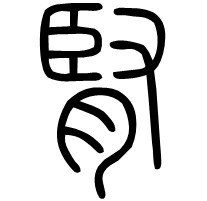
\includegraphics[width=\textwidth]{小篆/腎}
		\caption*{\content{腎}{腎(肾)}}
	\end{subcaptionblock}
	\caption{\content{《說文》小篆中的「月」與「肉」}{说文《小篆》中的“月”与“肉”}}
	\label{figure:《說文》小篆中的「月」與「肉」}
\end{figure}
\content{以「今文」釋漢字者不止王安石一人,漢朝的今文經學家們便是在用當時的隸書來解釋漢字。「土乙力為地」是把「地」字的筆畫拆開,「泉貨」也能拆作「白水真\footnote{古時「真」也寫作「眞」。把「貨」字的「人」旁拿掉,剩下的部分便與「眞」字十分相像。}人」,「董」字也能拆作「千里艸\footnote{「艸」是「草」的初文,作偏旁時寫作「艹」。}」,凡此種種,實在荒謬。古文經學家在文字解釋方面要更接近真相,起碼他們相信文字不是一成不變的。只可惜,漢人對古文字知之甚少,所以即便是古文經學派的代表作《說文》,也還是在用小篆來解說字形\footnote{以上參見唐䦨《中國文字學》第十九節〈什麼叫演化〉。}。}{以“今文”释汉字者不止王安石一人,汉朝的今文经学家们便是在用当时的隶书来解释汉字。“土乙力为地”是把“地”字的笔画拆开,“泉貨”也能拆作“白水真\footnote{古时“真”也写作“眞”。把“貨”字的“人”旁拿掉,剩下的部分便与“眞”字十分相像。}人”,“董”字也能拆作“千里艸\footnote{“艸”是“草”的初文,作偏旁时写作“艹”。}”,凡此种种,实在荒谬。古文经学家在文字解释方面要更接近真相,起码他們相信文字不是一成不变的。只可惜,汉人对古文字知之甚少,所以即便是古文经学派的代表作《说文》,也还是在用小篆来解说字形\footnote{以上参见唐兰《中国文字学》第十九节“什么叫演化”。}。}\par
\content{筆者曾見大新倉頡網站上有這樣一個例子,解釋「國」字的由來:「戈」意為動干戈、打戰;「口」意為人口、牲口;「一」意為打勝戰、一統天下;「囗」圍田地成「國」字。如果把這種拆「今文」的做法用在輸入法中,那倒是無可非議;但若是不負責任地隨便拆字,再把它說成是某字的「由來」,那就和王安石們沒什麼分別了。金文中的「國」就是「\includecharacter{金文/國}」,意思是以武器守衛領土,哪有什麼「一統天下」之說}{}
\content{今人手中的古文字材料遠比漢人豐富,所以對於漢人所犯的錯誤,今人可以根據這些資料來糾正。因此,我們若要以形釋義,更須留意古文字的寫法,甚至要拿不同時期的寫法作比對,才能最大程度地減少錯誤,免得詒笑大方。}{今人手中的古文字材料远比汉人丰富,所以对于汉人所犯的错误,今人可以根据这些资料来纠正。因此,我们若要以形释义,更须留意古文字的写法,甚至要拿不同时期的写法作比对,才能最大程度地减少错误,免得诒笑大方。}\par
\subsubsection{\content{《說文》與「六書」理論}{《说文》与“六书”理论}}
\begin{boxquote}{\content{《說文解字·序》}{《说文解字·序》}}
	\content{諸生競逐說字,解經誼,稱秦之隸書為倉頡時書,云:「父子相傳,何得改易!」乃猥曰:「馬頭人為長,人持十為斗,虫者,屈中也。」廷尉說律,至以字斷法:「苛人受錢,苛之字止句也。」若此者甚眾,皆不合孔氏古文,謬於〈史籀〉。俗儒鄙夫,翫其所習,蔽所希聞。不見通學,未嘗睹字例之條。怪舊埶而善野言,以其所知為秘妙,究洞聖人之微恉。}{诸生竞逐说字,解经谊,称秦之隶书为仓颉时书,云:“父子相传,何得改易!”乃猥曰:“马头人为长,人持十为斗,虫者,屈中也。”廷尉说律,至以字断法:“苛人受钱,苛之字止句也。”若此者甚众,皆不合孔氏古文,谬于《史籀》。俗儒鄙夫,玩其所习,蔽所希闻。不见通学,未尝睹字例之条。怪旧埶而善野言,以其所知为秘妙,究洞圣人之微恉。}
\end{boxquote}
\content{許慎是東漢時期古文經學的支持者。他反對今文經學家們出於各種目的胡亂解釋文字、經書的做法,認為經書必須依照古文、古義來解釋,於是在前人的基礎上,整理小篆、籀文、「古文」若干,為其注音、釋義,歷經二十餘載,終成《說文解字》(簡稱《說文》)一書。}{许慎是东汉时期古文经学的支持都。他反对今文经学家们出于各种目的胡乱解释文字、经书的做法,认为经书必须依照古文、古义增解释,于是在前人的基础上,整理小篆、籀文、“古文”若干,为其注音、释义、历经二十余载,终成《说文解字》(简称《说文》)一书。}\par
\content{《說文》是中國歷史上最早的字典。此前雖然也有人撰寫過字書,但是要麼像〈急就篇〉那樣只是排列一些常見文字作為識字書,既不注音也不釋義,如果沒有老師講解,就不可能學會;要麼像《爾雅》那樣只釋義,不注音;而最早的韻書(注音而不釋義)也是魏晉時期才有的。《說文》雖然每個條目都不長,但卻兼有字形、字義、字音三方面,且收字量之大前所未有,因此它是第一本真正的字典,也是後人研究先秦漢語的重要參考。本書中的很多字便是援引《說文》小篆字形作為參考的。}{《说文》是中国历史上最早的字典。此前虽然也有人撰写过字书,但是要么像《急就篇》那样只是排列一些常见文字作为识字书,既不注音也不释义,如果没有老师讲解,就不可能学会;要么像《尔雅》那样只释义,不注音;而最早的韵书(注音而不释义)也是魏晋时期才有的。《说文》虽然每个条目都不长,但却兼有字形、字义、字音三方面,且收字量之大前所未有,因此说它是第一本真正的字典。}\par
\content{《說文》原本已經散佚,今人無從看到它的原貌;但從後世的校訂本來看,《說文》的體例大致是:按部首排列各字;以小篆為主要字形,兼收籀文、古文;有釋義,注音,可能還會按「六書」理論分析形、音、義之間的關係。}{《说文》原本已经散佚,今人无从看到它的原貌;但从后世的校订本来看,《说文》的体例大致是:按部首排列各字;以小篆为主要字形,兼收籀文、古文;有释义,注音,可能还会按“六书”理论分析形、音、义之间的关系。}\par
\content{「六書」一詞,最早見於《周禮》:}{“六书”一词,最早见于《周礼》:}
\begin{boxquote}{\content{《周禮·地官司徒》}{《周礼·地官司徒》}}
	\content{保氏:掌諫王惡,而養國子以道。乃教之六藝:一曰五禮,二曰六樂,三曰五射,四曰五馭,五曰六書,六曰九數。}{保氏:掌谏王恶,而养国子以道。乃教之六艺:一曰五礼,二曰六乐,三曰五射,四曰五驭,五曰六书,六曰九数。}
\end{boxquote}
\content{其中「九數」是指九九乘法表;前四個都是可以顧名思義的內容。用現在的話說,「六藝」教的就是小學的社會、音樂、健體、數學課程,以及「六書」。}{其中“九数”是九九乘法表;前四个都是可以顾名思义的内容。用现在的话说,“六艺”教的就是小学的道法、音乐、体育、数学课程,以及“六书”。}\par
\content{《周禮》記載簡略,並未說明「六書」的名目。古文經學家們認為「六書」是所有漢字的統稱,古人通過某種規則把所有漢字分為六類,於是叫「六書」。因此他們想方設法要從文字中分出六種類別來,形成一套理論。後來許慎的說法被大多數人所接受:}{《周礼》记载简略,并未说明“六书”的名目。古文经学家们认为“六书”是所有汉字的统称,古人通过某种规则把所有汉字分为六类,于是叫“六书”。因此他们想方设法要从文字中分出六种类别来,形成一套理论。后来许慎的说法被大多数人所接受:}
\begin{boxquote}{\content{《說文解字·序》}{《说文解字·序》}}
	\centering
	\content{一曰指事。指事者,視而可識,察而見意,「上、下」是也。\\二曰象形。象形者,畫成其物,隨體詰詘,「日、月」是也。\\三曰形聲。形聲者,以事為名,取譬相成,「江、河」是也。\\四曰會意。會意者,比類合誼,以見指撝,「武、信」是也。\\五曰轉注。轉注者,建類一首,同意相受,「考、老」是也。\\六曰假借。假借者,本無其事,依聲託事,「令、長」是也。}{一曰指事。指事者,视而可识,察而见意,“上、下”是也。\\二曰象形。象形者,画成其物,随体诘诎,“日、月”是也。\\三曰形声。形声者,以事为名,取譬相成,“江、河”是也。\\四曰会意。会意者,比类合谊,以见指撝,“武、信”是也。\\五曰转注。转注者,建类一首,同意相受,“考、老”是也。\\六曰假借。假借者,本无其事,依声托事,“令、长”是也。}
\end{boxquote}
\content{古文經學家們崇古(甚至於媚古),所以在由漢至清的兩千年裡,人們總是把《說文》中的「六書」理論奉為圭臬\footnote{至於今文經學家,他們的理論大概更靠不住。也許連與他們有關的笑話都失傳了。}。也有少數人發現了「六書」理論的不足而予以修補,卻仍未跳出「六書」的理論框架。至於對其做出系統性的批判和反思,那都是近現代的事了。}{古文经学家们崇古(甚至于媚古),所以在由汉至清的两千年里,人们决是把《说文》中的“六书”理论奉为圭臬\footnote{至于今文经学家,他们的理论大概更靠不住。也许连与他们有关的笑话都失传了。}。也有少数人发现了“六书”理论的不足而予以修补,却仍未跳出“六书”的理论框架。至于对其做出系统性的批判和反思,那都是近现代的事了。}\par
\content{筆者認為,與「六書」有關的問題主要有以下幾個方面:}{笔者认为,与“六书”有关的问题主要有以下方面:}
\begin{enumerate}
	\item \content{《周禮》中的「六書」到底是指什麼?漢人把它說成是「漢字分類法」乃至「造字之本」,這真的可信嗎?今人已對這方面有些研究,如張政琅認為「六書」其實是「六甲」,即天干地支之學\footnote{參看張政琅\href{https://www2.ihp.sinica.edu.tw/file/4848wQZFtQw.pdf}{〈六書古義〉}。}。如果「六書」本身就不是什麼汉字分类法,那麼漢人一定要湊出「六」種類別,豈不荒謬?}{《周礼》中的“六书”到底是指什么?汉人把它说成是“汉字分类法”乃至“造字之本”,这真的可信吗?今人已对这方面有些研究,如张政琅认为“六书”其实是“六甲”,即天干地支之学\footnote{参看张政琅\href{https://www2.ihp.sinica.edu.tw/file/4848wQZFtQw.pdf}{《六书古义》}。}。如果“六书”本身就不是什么汉字分类法,那么汉人一定要湊出“六”种类别,岂不荒谬?}
	\item \content{退一步講,即便漢字真的可以分成六類,但許慎所做的也只是對當時能見到的古漢字的「總結」,完全談不上是造字的「方法」或「原則」。有人說「中國文字在小篆以前仍然遵從『六書』造字原則,漢隸則不再遵守『六書』原則,自行變化造形」,筆者認為這並不奇怪,因為「六書」本來就是透過小篆以前的文字總結出來的,小篆以前的文字自然符合這種後驗理論;但這種後驗理論卻不能預測將來的文字演變,所以面對漢隸及以後的字就失靈了。\footnote{所以更嚴謹的說法應該是:「『六書』理論較好地貼合了小篆以前文字的演變過程;但漢隸以後的文字卻是朝著另一個不同於『六書』的方向演變下去了。」}}{退一步讲,即便汉字真的可以分成六类,但许慎所做的也只是对当时能见到的古汉字的“总结”,完全谈不上是造字的“方法”或“原则”。有人说“中国文字在小篆以前仍然遵从‘六书’造字願是,汉隶则不再遵守‘六书’原则,自行变化造形”,笔者认为这并不奇怪,因为“六书”本来就是通过小篆以前的文字总结出来的,小篆以前的文字自然符合这种后验理论;但这种后验理论却不能预测将来的文字演变,所以面对汉隶及以后的字就失灵了。\footnote{所以更严谨的说法应该是:“‘六书’理论较好地结合了小篆以前文字的演变过程;但汉隶以后的文字却是朝着另一个不同于‘六书’的方向演变下去了。”}}
	\item \content{再退一步講,即便只總結小篆以前的文字,許慎們也沒有獲取到足夠多的資料。漢人不知道甲骨文,也沒有見到多少金文,還誤判了「古文」的所處時代,那麼基於這些不夠全面還有些許錯誤的資料,真的能還原出「造字理論」的全貌嗎?筆者覺得這也是要打一個問號的——畢竟,有些本來看甲骨文可以很容易解釋通的字,看小篆卻可能解釋不清了\footnote{參見後文「訛變」一小節。}。}{再退一步讲,即便只总结小篆以前的文字,许慎们也没有获取到足够多的资料。汉人不知道甲骨文,也没有见到多少金文,还误判了“古文”的所处时代,那么基于这些不够全面还有些许错误的资料,真的能还原出“造字理论”的全貌吗?笔者觉得这是要打一个问号的——毕竟,有些本来看甲骨文可以奶容易解释通的字,看小篆却可能解释不清了\footnote{参见后文“讹变”一小节。}。}
	\item \content{最後再退一步講,即便許慎的「六書」理論很完善,很成熟,但許慎本人卻沒有詳加解釋,而他給出的廖廖十二個字例中,有些很模糊,有些又不對,以致後人對其中的很多名目都有爭議——這也是近現代人批判「六書」時最主要的著眼點。六書中的「轉注」是爭議最大的,光是裘錫圭在《文字學概要》中就整理了九種不同的說法。實際的異說想必更多,大有「百家爭鳴」之局面。}{最后再退一步讲,即便许慎的“六书”理论很完善,很成熟,但许慎本人却没有详加解释,而他给出的廖廖十二个字例中,有些很模糊,有些又不对,以致后人对其中的很多名目都有争议——这也是近现代人批判“六书”时最主要的着眼点。六书中的“转注”是争议最大的,光是裘锡圭在《文字学概要》中就整理了九种不同的说法,实际的异说想必理多,大有“百家争鸣”之局面。}
\end{enumerate}\par
\content{筆者認為,「六書」理論的基礎本來就有這樣或那樣的疑點,許慎說明「六書」時又沒有解釋得足夠清晰——更何況哪怕真的解釋清晰了也未必見得正確。所以,今人在研究古文字時,不應再囿於「六書」那套話語體系了。人們只需取「六書」中有價值的部分,比如界定得比較清晰的「形聲」,這個概念仍為現代理論所用;至於其它界定不明的部分,現代人應該有自己的思考,大可不必抓著「象形」「指事」「會意」「轉注」這些概念爭執不休。}{笔者认为,“六书”理论的基础本来就有这样或那样的疑点,许慎说明“六书”时又没有解释得足够清晰——更何况哪怕真的解释清晰了也未必见得正确。所以,今人在研究古文字时,不应再囿于“六书”那套话语体系了。人们只需取“六书”中有价值的部分,比如界定得比较清晰的“形声”,这个概念仍为现代理论所用;至于其它界定不明的部分,现代人应该有自己的思考,大可不必抓着“象形”“指事”“会意”“转注”这些概念争执不休。}\par
\subsection{\content{漢字演變過程中的現象}{汉字演变过程中的现象}}\label{subsection:漢字演變過程中的現象}
\content{有些人對漢字演變的過程不了解,以為漢字的演變是線性的:先有甲骨文,再有金文,然後依次是大篆\footnote{「大篆」這個概念被人们用得非常亂,不同的人有不同的定義。為了明確起見,本書不使用「大篆」這一名稱。}、小篆、隸書、楷書、行書、草書,都是後一種書體繼承前一種。但真實的情況是,這些書體之間有著複雜的網狀關係。}{有些人对汉字演变的过程不了解,以为汉字的演变是线性的:先有甲骨文,再有金文,然后依次是大篆\footnote{“大篆”这个概念被人们用得非常乱,不同的人有不同的定义。为了明确起见,本书不使用“大篆”这一名称。}、小篆、隶书、楷书、行书、草书,都是后一种书体继承前一种。但真实的情况是,这些书体之间有着复杂的网状关系。}\par
\content{可惜限於篇幅,正文這裡不能細講漢字的演變過程;本節我們只來談漢字演變過程中的現象。讀者若是想要了解漢字演變的大致過程,可以參考筆者在\cref{appendix:evolution of chinese characters}中根據一些資料整理的漢字演變圖譜。}{可惜限于篇幅,正文这里不能细讲汉字的演变过程;本节我们只来谈汉这演变过程中的现象。读者若是想要了解汉字演变的大致过程,可以参考笔者在\cref{appendix:evolution of chinese characters}中根据一些资料整理的汉字演变图谱。}\par
\subsubsection{\content{並行的正體與俗體}{并行的正体与俗体}}
\content{在分裂割據時期,像戰國那樣不同字體並行的情況不足為奇;而在統一王朝時期,不同字體並行的情況也並不鮮見。商代後期有甲骨文和金文並行,秦朝有小篆和隸書並行,西漢則有隸書和章草\footnote{章草,草書的一種,是由隸書演變而來的。我們一般所說的「草書」是指今草,它是由楷書演變而來的。章草與今草有不少差異。}並行。今人使用的各種印刷字體,比如明體、楷體、仿宋體、黑體等,未嘗不可看作並行書體;但是我們還是把眼光放到古代的手寫體上吧。}{在分裂割据时期,像战国那样不同字体并行的情况不足为奇;而在统一王朝时期,不同字体并行的情况也并不鲜见。商代后期有甲骨文和金文并行,秦朝有小篆和隶书并行,西汉则有隶书和章草\footnote{章草,草书的一种,是由隶书演变而来的。我们一般所说的“草书”是指今草,它是由楷书演变而来的。章草与今草有不少差异。}并行。今人使用的各种印刷字体,比如宋体、楷体、仿宋体、黑体等,未尝不可看作并行书体;但是我们还是把眼光放到古代的手写体上吧。}\par
\content{統一王朝時期並行的字體通常不會有太大差異,相似之處很多\footnote{原因顯而易見。若是要讓甲骨文和現代楷書並行的話,人們要學習兩套全然不同的書寫形式,這樣的並行就只能成為一種負擔。}。就以甲骨文和商代金文來說,它們的寫法大致相似,見\cref*{table:一些漢字的商金文與甲骨文}。}{统一王朝时期并行的字体通常不会有太大差异,相似之处很多\footnote{原因显而易见。若是要让甲骨文和现代楷书并行的话,人们要学习两套全然不同的书写形式,这样的并行就只能成为一种负担。}。就以甲骨文和商代金文来说,它们的写法大致相似,见\cref*{table:一些漢字的商金文與甲骨文}。}\par
\begin{table}[H]
	\centering
	\caption{\content{一些漢字的商金文與甲骨文}{一些汉字的商金文与甲骨文}}
	\label{table:一些漢字的商金文與甲骨文}
	\begin{NiceTabular}{*{7}{c}}[hlines]
	\CodeBefore
		\rowcolor{lightgray}{1}
		\columncolor{lightgray}{1}
	\Body
		\toprule
		\content{現代漢字}{现代汉字} & 天 & 鳥\content{}{(鸟)} & 兒\content{}{(儿)} & 女 & 止 & 韋\content{}{(韦)}\\\midrule[.6pt]
		\Block[m]{}{商金文} & \includegraphics[width=3.5em]{金文/天} & \includegraphics[width=3.5em]{金文/鳥} & \includegraphics[width=3.5em]{金文/兒} & \includegraphics[width=3.5em]{金文/女} & \includegraphics[width=3.5em]{金文/止} & \includegraphics[width=3.5em]{金文/韋}\\
		\Block[m]{}{甲骨文} & \includegraphics[width=3.5em]{甲骨文/天} & \includegraphics[width=3.5em]{甲骨文/鳥} & \includegraphics[width=3.5em]{甲骨文/兒} & \includegraphics[width=3.5em]{甲骨文/女} & \includegraphics[width=3.5em]{甲骨文/止} & \includegraphics[width=3.5em]{甲骨文/韋}\\\bottomrule
	\end{NiceTabular}
\end{table}
\content{比較一下便很容易看出來,金文筆畫流暢,細節豐富,字跡端莊,似是毛筆筆法\footnote{實際上金文不是直接由毛筆寫在青銅器上的,因為青銅器上的銘文都是凹入器皿中的,顯然需要在製造模具時便用某種方式把文字附在模具之上。至於銘文究竟是以何種方式「寫」在青銅器上,這中間又是否有毛筆的參與,今人已不得而知。};甲骨文則是典型的刀筆字,直筆較多,曲筆較少,筆畫轉折處時常拆作兩筆來寫,且每個字的筆畫粗細很一致。}{比较一下便很容易看出来,金文笔画流畅,细节丰富,字迹端庄,似是毛笔笔法\footnote{实际上金文不是直接由毛笔写在青铜器上的,因为青铜器上的铭文者是凹入器皿中的,显然需要在制造模具时便用某种方式把文字附在模具之上。至于铭文究竟是以何种方式“写”在青铜器上,这中间又是否有毛笔的参与,今人已不得而知。};甲骨文则是典型的刀笔字,直笔较多,曲笔较少,笔画转折处时常拆作两笔来写,且每个字的笔画粗细很一致。}\par
\content{書寫工具的差異確實可以解釋一些現象,比如「止」字的甲骨文要比金文簡陋一些。但是它解釋不了,為什麼「韋」的金文是四個「止」,而甲骨文卻只有兩個「止」\footnote{很多甲骨文的寫法不固定。就以「韋」字為例,除了上表所列之字外,筆者還查到有三個「止」的「\includecharacter{甲骨文/韋1}」和兩個「止」分列左右的「\includecharacter{甲骨文/韋2}」。另外,從西周金文開始,「韋」字便用兩「止」了,寫成「\includecharacter{金文/韋1}」,顯然是正體字吸收了俗體字的寫法。}。這種甲骨文比同時期金文簡省部件的現象比比皆是,我們很難牽強附會地把原因歸結為書寫工具的差異。}{书写工具的差异确实可以解释一些现象,比如“止”字的甲骨文要比金文简陋一些。但是它解释不了,为什么“韦”的金文是四个“止”,而甲骨文却只有两个“止”\footnote{很多甲骨文的写法不固定。就以“韦”字为例,笔者还查到有三个“止”的「\includecharacter{甲骨文/韋1}」和两个“止”分列左右的「\includecharacter{甲骨文/韋2}」。另外,从西周金文开始,“韦”字便用两“止”了,写成「\includecharacter{金文/韋1}」,显然是正体字吸收了俗体字的写法。}。这种甲骨文比同时期金文简省部件的现象比比皆是,我们很难牵强附会地把原因归结为书写工具的差异。}\par
\content{真正的原因在於使用埸合。商代青銅器貴重,且生產流程複雜,只能用在比較鄭重的場合下,所以人們「寫」金文時不敢怠慢,要寫得非常標準,更不會為了嫌麻煩而簡省部件。但在日常生活中,人們要使用甲骨及竹簡書寫大量內容,自然會對筆畫繁複的字感到厭煩,於是有意或無意地簡省部件,只要保證還能看懂即可。用於正式場合的\textbf{正體}和用於非正式場合的\textbf{俗體}便是這樣分道揚鑣的。}{真正的原因在于使用场合。商代青铜器贵重,且生产流程复杂,只能用在比较郑重的场合下,所以人们“写”金文时不敢怠慢,要写得非常标准,更不会为了嫌麻烦而简省部件。但在日常生活中,人们要使用甲骨及竹简书写大量内容,自然会对笔画繁复的字感到厌烦,于是有意或无意地简省部件,只要保证还能看懂即可。用于正式场合的\textbf{正体}和用于非正式场合的\textbf{俗体}便是这样分道扬镳的。}\par
\content{秦朝以小篆為正體,官方文件皆使用小篆。隸書的書寫效率高於小篆,所以底層公務員們當然願意使用隸書,隸書便是秦朝的俗體。到了西漢,隸書逐漸取代小篆,成為正體;而由隸書發展而來的、書寫效率更高的章草則作為俗體存在。唐朝及以後的正體一般都是楷書,而俗體主要是行書。}{秦朝以小篆为正体,官方文件皆使用小篆。隶书的书写效率高于小篆,所以底层公务员们当然愿意使用隶书,隶书便是秦朝的俗体。到了西汉,隶书逐渐取代小篆,成为正体;而由隶书发展而来的、书写效率更高的章草则作为俗体存在。唐朝及以后的正体一般都是楷书,而俗体主要是行书。}\par
\subsubsection{\content{假借}{假借}}
\content{正如我們在\cref{section:bopomofo-pinyin}開首所說的那樣,我們學習語言都是先學會「音」再學會「形」的。那麼對於一個漢語使用者(尤其是初學者)來說,如果在寫作時遇到只會唸不會寫的漢字,卻又沒有字典可查,他會怎麼辦呢?}{正如我们在\cref{section:bopomofo-pinyin}开首所说的那样,我们学习语言都是先学会“音”再学会“形”的。那么对于一个汉语使用者(尤其是初学者)来说,如果在写作时遇到只会念不会写的汉字,却又没有字典可查,他会怎么办呢?}\par
\content{一種解決方法是,用注音符號/漢語拼音來表示這個字。我們假想,如果此人連一個漢字都不會寫,只會拼音的話,那麼他寫出來的文章將是通篇的拼音文字。作為拼音文字的各種歐文便是這樣形成的:只需要把表音的字母排起來,就可以表示人們話語中的每個詞,甚至是非人的拟聲詞,比如meow。}{一种解决方案是,用注音符号/汉语拼音来表示这个字。我们假想,如果此人连一个汉字都不会写,只会拼音的话,那么他写出来的文章将是通篇的拼音文字。作为拼音文字的各种欧文便是这样形成的:只需要把表音的字母排起来,就可以表示人们话语中的每个词,甚至是非人的拟声词,比如meow。}\par
\content{另一種解決方案是,找個會寫的同音字,乃至音近字來替代。這種現象直到今天還存在,一個人因為提筆忘字或什麼別的原因而把一字誤寫成同音的另一字,是再正常不過的事。}{另一种解决方案是,找个会写的同音字,乃至音近字来替代。这种现象直到今天还存在,一个人因为提笔忘字或什么别的原因而把一字误写成同音的另一字,是再正常不过的事。}\par
\content{而在漢字形成的早期,古人遇到的問題可不是「提筆忘字」那麼簡單,而是「想表達某個意思,卻沒有這個字」。為了解決這個問題,人們可以採用的方法主要有這樣幾種:}{而在汉字形成的早期,古人遇到的问题可不是“提笔忘字”那么简单,而是“想表达某个意思,却没有这个字”。为了解决这个问题,人们可以采用的方法主要有这样几种:}
\begin{description}
	\item[\content{表意造字}{表意造字}] \content{早期漢字的象形程度比較高,很多有形貌的實物都可以用圖畫的方式表現出來,所以乾脆造新字就行,比如「羊」在甲骨文中作「\includecharacter{甲骨文/羊}」,「犬」在商金文中作「\includecharacter{金文/犬}」。}{早期汉字的象形程度比较高,很多有形貌的实物都可以用图画的方式表现出来,比如“羊”在甲骨文中作“\includecharacter{甲骨文/羊}”,“犬”在商金文中作“\includecharacter{金文/犬}”。}
	\item[\content{形聲造字}{形声造字}] \content{當漢字量達到一定規模,並且漢字的象形程度逐漸降低\footnote{隸書以後的漢字幾乎完全不象形了。}之後,造表意字的難度就很高了。但造形聲字卻會隨著漢字量的增加變得更簡單。但在實際中,直接形聲造字的情況是少見的,假借的情況更多。}{当汉字量达到一定规模,并且汉字的象形程度逐渐降低\footnote{隶书以后的汉字几乎完全不象形了。}之后,造表意字的难度就很高了。但造形声字却会随着汉字量的增加变得更简单。但在实际中,直接形声造字的情况是少见的,假借的情况更多。}
	\item[\content{假借用字}{假借用字}] \content{有形貌的實物勉強還可以畫出來,但是沒有形貌的虛詞,如「我」「其」「它」「無」等等,怎麼可能畫得出來呢?為了書寫這些虛詞,古人常常借用同音或音近的詞來表示,這就是最典型的假借現象。這種方法同樣可以用於表示新生事物。}{有形貌的实物勉强还可以画出来,但是没有形貌的虚词,如“我”“其”“它”“无”等等,怎么可能画得出来呢?为了书写这些虚词,古人常常借用同音或音近的词来表示。这种方法同样可以用于表示新生事物。}
\end{description}\par
\content{「它」的本義是蛇,金文作「\includecharacter{金文/它}」,形狀極像一條蛇。這兩字在上古音中是同一韻母的,發音比較接近,所以人們借「\includecharacter{金文/它}」表示「它」的含義;而後為了區分這兩個意思,又為名詞含義的字加了「虫」旁\footnote{古時「蟲」的含義很寬,包括各種動物。人們還根據體表特徵,把各種動物(包括人)分為「五蟲」:裸蟲、毛蟲、羽蟲、鱗蟲、甲蟲。},於是「它」字就不再用作名詞了,只用作代詞。}{“它”的本义是“蛇”,金文作“\includecharacter{金文/它}”,形状极像一条蛇。这两字在上古音中是同一韵母的,发音比较接近,所以人们借“\includecharacter{金文/它}”表示“它”的含义;而后为了区分这两个意思,又为名词含义的字加了“虫”旁\footnote{古时“虫”的含义很宽,包括各种动物。人们还根据体表特征,把各种动物(包括人)分为“五虫”:裸虫、毛虫、羽虫、鳞虫、甲虫。},于是“它”字就不再用作名词了,只用作代词。}\par
\content{「無」本來與「舞」是同一字,甲骨文作「\includecharacter{甲骨文/舞}」,表示人手持某物跳舞。同样地,因為「\includecharacter{甲骨文/舞}」字與口語中的「無」音近,人們就借它來表示「無」的含義。}{“无”(繁体为“無”)本来与“舞”是同一字,甲骨文作“\includecharacter{甲骨文/舞}”,表示人手持某物跳舞。因为“\includecharacter{甲骨文/舞}”字与口语中的“无”音近,人们就借它来表示“无”的含义。}\par
\content{類似的還有「其」假借「箕」(商金文作「\includecharacter{金文/其}」),「我」假借某種兵器名(已不可考;春秋金文作「\includecharacter{金文/我}」),《論語》中還假借「說」字來表示「悅」字的含義\footnote{「子曰:『學而時習之,不亦說乎?』」},諸如此類,不勝枚舉。}{类似的还有“其”假借“箕”(商金文作“\includecharacter{金文/其}”),“我”假借某种兵器名(已不可考;春秋金文作“\includecharacter{金文/我}”),《论语》中还假借“说”字来表示“悦”的含义\footnote{“子曰:‘学而时习之,不亦说乎?’”},诸如此类,不胜枚举。}\par
\begin{wrapfigure}{O}{.2\textwidth}
	\centering
	\begin{tikzpicture}
		\begin{scope}
			\clip(0,0)rectangle(2.6,11.9);
			\node[inner sep=0pt]at(-1.4,6){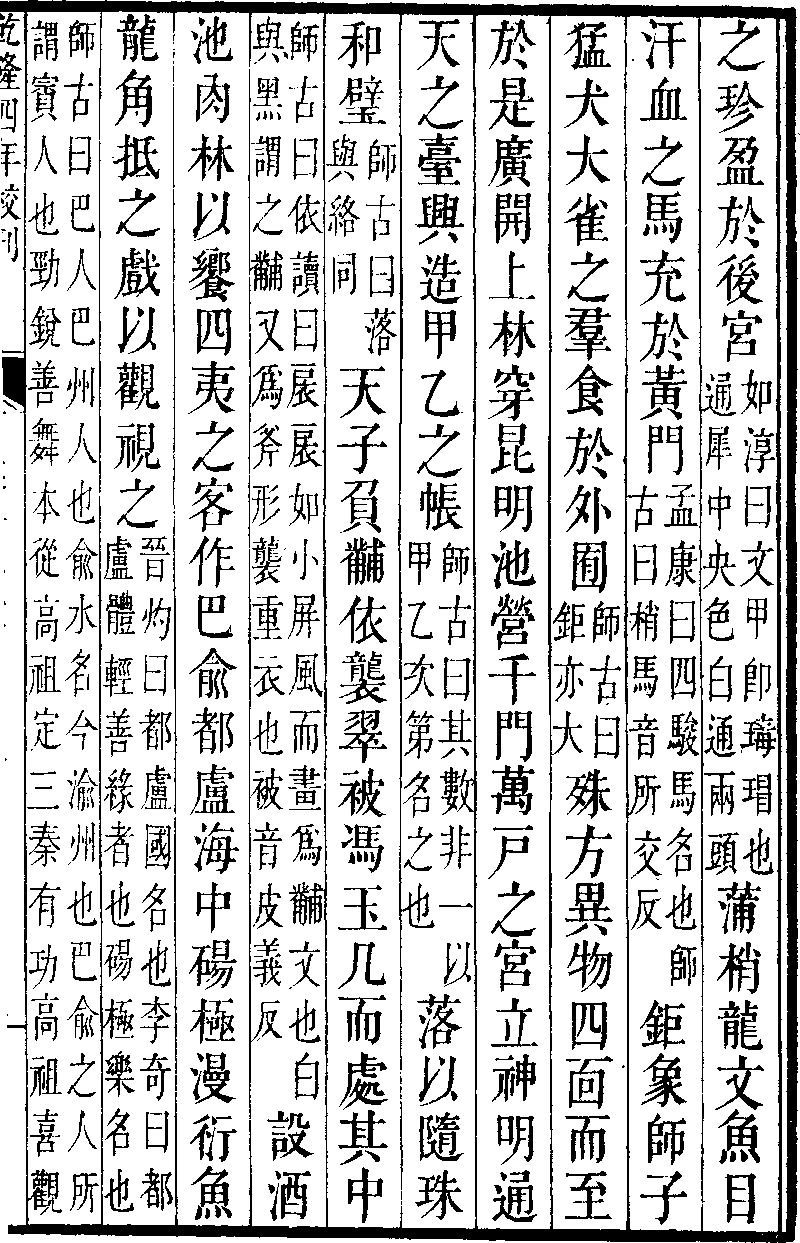
\includegraphics[height=12cm]{漢書-西域傳下-師子.png}};
		\end{scope}
		\draw[red](.9,.15)rectangle(1.45,1.3);
	\end{tikzpicture}
	\caption{\content{《漢書》中的「師子」}{《汉书》中的“师子”(師子)}}
	\label{figure:《漢書》中的「師子」}
\end{wrapfigure}
\content{名詞同樣可以假借別字來表示。古人通西域以前不知道獅子,所以漢語中原本沒有獅子對應的表意字。彼時隸書已經十分成熟,新造象形字並不現實,所以漢人起初就假借「軍隊」之意的「師」字表示獅子。《漢書》記載西域動物時便是寫作「師子」(\cref*{figure:《漢書》中的「師子」})。直到近代,假借都始終是翻譯舶來詞的重要手段。從清末到民國初年,僅coffee一詞就有「加非」「磕肥」「高馡」「考非」等各種譯名,這些譯名顯然都是同音(近音)假借的產物。}{名词同样可以假借别字来表示。古人通西域以前不知道狮子,所以汉语中原本没有狮子对应的表意字。彼时隶书已经十分成熟,新造象形字并不现实,所以汉人起初就假借“军队”之意的“師”(师)来表示狮子。《汉书》记载西域动物时便是写作“師子”(\cref*{figure:《漢書》中的「師子」})。直到近代,假借都始终是翻译舶来词的重要手段。从清末到民国初年,仅coffee一词就有“加非”“磕肥”“高馡”“考非”等各种译名,这些译名显然都是同音(近音)假借的产物。}\par
\content{日文中的假借現象更普遍,甚至有專門的假名系統來表音——這裡的「假」字正是「假借」之意。}{日文中的假借现象更普遍,甚至有专门的假名系统来表音——这里的“假”字正是“假借”之意。}\par
\subsubsection{\content{形聲字}{形声字}}
\content{假借的方法十分方便,不需要另行造字,所以在漢字發展的過程中始終起著重要的作用。但是,假借的濫用會導致很多同形、同音的異義字出現。如果這樣的字太多,我們就需要在閱讀時猜每個字的意思,既讀得很慢,又容易犯錯。}{假借的方法十分方便,不需要另行造字,所以在汉字发展的过程中始终起着重要的作用。但是,假借的滥用会导致很多同形、同音的异义字出现。如果这样的字太多,我们就需要在阅读时猜每个字的意思,既读得很慢,又容易犯错。}\par
\content{為了克服這樣的問題,人們又在慢慢地改造漢字,以此分化多義字,減少歧義。「它」的本義是蛇,之後被借來用作代詞。為了區分本義和假借義,人們為「它」字加注了一個「虫」旁,寫成「蛇」,這個過程就是把本義分化出去了。「師」的本義是「軍隊」「老師」或作官名,漢朝時曾被借來表示獅子。後來人們為「師」字加注了一個「犭」旁,寫成「獅」,這個過程就是把假借義分化出去了。}{为了克服这样的问题,人们又在慢慢地改造汉字,以此分化多义字,减少歧义。“它”的本义是蛇,之后被借来用作代词。为了区分本义和假借义,人们为“它”字加注了一个“虫”旁,写成“蛇”,这个过程就是把本义分化出去了。“師”(师)字的本义是“军队”“老师”或作官名,汉朝时曾被借来表示狮子。后来人们为“師”字加注了一个“犭”旁,写成“獅”(狮),这个过程就是把假借义分化出去了。}\par
\content{以上兩種情況是在已有的文字上加注表意符號的例子——加「虫」表示動物,加「犭」表示兽。還有些情況下人們會加注表音符號,透過不同的音來區分不同的字。舉個例子,「金」字的本義可以指各種金屬\footnote{周以前各種金屬都叫「金」,所以刻在青銅器上的銘文當然叫「金文」而不是「銅文」。},後來隨著人們對金屬的知識逐漸豐富,金屬也分成了金、鐵、錫、銅、銀等多種類型。為了從字形上區分不同金屬,人們就可以為「金」加注「易」旁表示錫,加注「同」旁表示銅,加注「艮」旁表示銀,諸如此類。}{以上两种情况是在已有的文字上加注表意符号的例子——加“虫”表示动物,加“犭”表示兽。还有些情况下人们会加注表音符号,通过不同的音来区分不同的字。举个例子,“金”字的本义可以指各种金属\footnote{周以前各种金属都叫“金”,所以刻在青铜器上的铭文当然叫“金文”而不是“铜文”。},后来随着人们对金属的知识逐渐丰富,金属也分成了金、铁、锡、铜、银等多种类型。为了从字形上区分不同金属,人们就可以为“金”加注“易”旁表示锡,加注“同”旁表示“铜”,加注“艮”旁表示银,诸如此类。}\par
\content{以上所舉都是形聲字。顧名思義,形聲字既有表意的成分——形旁,又有表音的成分——聲旁。人們看到形聲字後便可根據形旁大致猜測其意義,根據聲旁大致猜測其讀音\footnote{因為各種複雜的原因,如今我們想要憑借形聲字的聲旁來猜讀音常常是不準確的。但是不少形聲字的讀音仍與其聲旁有一定關聯。}。是「馬」字作形旁或作聲旁的一些文字,其中有些字是先秦時沒有的,如「螞」,這個字大概很晚才出現,但卻是很典型的形聲字。}{以上所举都是形声字。顾名思义,形声字既有表意的成分——形旁,又有表音的成分——声旁。人们看到形声字后便可根据形旁大致猜测其意义,根据声旁大致猜测其读音\footnote{因为各种复杂的原因,如今我们想要凭借形声字的声旁来猜读音常常是不准确的。但是不少形声字的读音仍其声旁有一定关联。}。是“马”(馬)字作形旁或作声旁的一些文字释义,其中有些字是先秦时没有的,如“蚂”,这个字大概很晚才出现,但却是很典型的形声字。}\par
\begin{table}[H]
	\centering
	\caption{\content{「馬」相關的部分形聲字}{“马”相关的部分形声字}}
	\label{table:「馬」相關的部分形聲字}
	\begin{NiceTabular}{*{8}{c}}[hlines]
	\CodeBefore
			\rowcolor{lightgray}{1}
			\cellcolor{red!25}{1-6}
			\cellcolor{blue!25}{1-8}
			\columncolor{lightgray}{1}
			\columncolor{red!25}{5}
			\columncolor{blue!25}{7}
	\Body
		\toprule
		\content{形聲字}{形声字} & \content{古字形}{古字形} & \content{古義}{古义} & \content{古音}{古音} & \content{形旁}{形旁} &\content{古義}{古义} & \content{聲旁}{声旁} & \content{古音}{古音} \\\midrule[.6pt]
		\content{螞}{蚂(螞)} & & \content{蟲名}{虫名} & \content{莫下切}{莫下切} & \content{虫(蟲)}{虫} & \content{動物}{动物} & \Block{2-1}{\content{馬}{马(馬)}} & \Block{2-1}{\content{莫下切}{莫下切}} \\
		\content{䣕}{䣕} & \includecharacter{小篆/䣕} & \content{地名}{地名} & \begin{tabular}{c} \content{莫下切}{莫下切} \\ \content{莫駕切}{莫驾切} \end{tabular} & \content{⻏(邑)}{⻏(邑)} & \content{城}{城} \\
		\content{驚}{惊(驚)} & \includecharacter{小篆/驚} & \content{馬受刺激}{马受刺激} & \content{舉卿切}{举卿切} & \Block{3-1}{\content{馬}{马(馬)}} & \Block{3-1}{\content{馬}{马}} & \content{敬}{敬} & \content{居慶切}{居庆切} \\
		\content{駭}{骇(駭)} & \includecharacter{小篆/駭} & \content{受驚}{受惊} & \content{侯楷切}{侯楷切} & & & \content{亥}{亥} & \content{胡改切}{胡改切} \\
		\content{驀}{蓦(驀)} & \includecharacter{小篆/驀} & \content{上馬}{上马} & \content{莫白切}{莫白切} & & & \content{莫}{莫} & \content{慕各切}{慕各切} \\\bottomrule
 	\end{NiceTabular}
\end{table}
\content{形聲字多且混亂,常常隨著人們的需要而發生變化。例如,作為戰爭武器的炮原本是寫作「砲」或「礮」\footnote{從中國甲午戰爭博物院現存的光緒二十年(1894)二月二十五日李鴻章奏折中可以看出,當時的公文中尚用「礮」字表示火炮。可見「石」旁的炮字直至清末還在使用。}的,因為最早的炮就是投石機;後來火虊出現,火虊炮慢慢取代了機械炮,後人就把「石」旁的「砲」字改為「火」旁的「炮」\footnote{另,古時「炮」字便已存在,但彼時的含義只是「火烤」,如古代死刑「炮烙」;沒有作為武器的含義。按裘錫圭的說法,古時的「炮」和後來作武器的「炮」是字形相同的兩個不同的字(同形字)。},再之後「炮」字就被廣泛接受而成為正體了。}{形声字多且混乱,常常随着人们的需要而发生变化。例如,作为战争武器的炮原本是写作“砲”或“礮”的\footnote{从中国甲午战争博物院现存的光绪二十年(1894)二月二十五日李鸿章奏折中可以看出,当时的公文中尚用“礮”字表示火炮。可见“石”旁的炮字直至清末还在使用。}的,因为最早的炮就是投石机;后来火药出现,火药炮慢慢取代了机械炮,后人就把“石”旁的“砲”字改为“火”旁的“炮”\footnote{另,古时“炮”字便已存在,但彼时的含义只是“火烤”,如古代死刑“炮烙”;没有作为武器的含义。按裘锡圭的说法,古时的“炮”和后来作武器的“炮”是字形相同的两个不同的字(同形字)。},再之后“炮”字就被广泛接受而成为正体了。}\par
\content{大多數形聲字都不是憑空產生的。它們往往是透過改造已有文字得來的,這其中隱含著漫長的發展過程。當然也不乏一些由人們直接挑選形旁聲旁組出來的形聲字,比如徐壽在翻譯化學元素名時造了若干「金」旁的字;朱元璋的子孙們更是貢獻了不少形聲字\footnote{朱元璋規定,後代人取名時,第二字的偏旁必須依「木火土金水」的順序取。古人又有避諱的習俗,祖上用過的字不能再用,漸漸地就無字可用了,便去發掘古籍中的生僻字,甚至乾脆自行造字。這些新字多數是以「木火土金水」為形旁的形聲字。}。}{大多数形声字都不是凭空产生的。它们往往是通过改造已有文字得来的,这其中隐含着漫长的发展过程。当然也不乏一些由人们直接挑选形旁声旁组出来的形声字,比如徐寿在翻译化学元素名时造了若干“金”旁的字;朱元璋的子孙们更是贡献了不少形声字\footnote{朱元璋规定,后代人取名时,第二字的偏旁必须依“木火土金水”的顺序取。古人又有避讳的习俗,祖上用过的字不能再用,渐渐地就无字可用了,便去发掘古籍中的生僻字,甚至干脆自行造字。这些新字多数是以“木火土金水”为形旁的形声字。}。}\par
\subsubsection{\content{異體字}{异体字}}
\begin{boxquote}{\content{《吶喊·孔乙己》}{《呐喊·孔乙己》}}
	\content{孔乙己顯出極高興的樣子,將兩個指頭的長指甲敲着櫃臺,點頭說,「對呀對呀!……回字有四樣寫法,你知道麼?」}{孔乙己显出极高兴的样子,将两个指头的长指甲敲着柜台,点头说,“对呀对呀!……回字有四样写法,你知道么?”}
\end{boxquote}
\content{\cref*{figure:「隱」字的早期寫法}是秦漢時期「隱」字的各個寫法。不同時期的字在筆畫形態上有些差異,比如「爫」可能寫作「⺈」\footnote{在漢字發展過程中,「爫」「⺈」相混、「爫」「𱼀」相混、「⼑」「⺈」相混都是很常見的,比如「爭」與「争」、「摇」與「搖」、「絕」與「絶」等。},這點我們姑且不論。更關鍵的差異在於部件:在某些寫法中,「爫」與「⺕」間有一個「工」;但在另一些寫法中就沒有。今天台灣的正體字作「隱」而中國大陸的簡體字作「隐」,原来這兩種寫法都有很深的淵源!}{\cref*{figure:「隱」字的早期寫法}是秦汉时期“隐”字的各个写法。不同时期的字在笔画形态上有些差异,比如“爫”可能写作“⺈”\footnote{在汉字发展过程中,“爫”“⺈”相混、“爫”“𱼀”相混、“⼑”“⺈”相混都是很常见的,比如“爭”与“争”、“摇”与“搖”、“絕”与“绝”等。},这点我们姑且不论。更关键的差异在于部件:在某些写法中,“爫”与“⺕”间有一个“工”;但在另一些写法中就没有。今天台湾的繁体字作“隱”而中国大陆的简体字作“隐”,原来这两种写法都有很深的渊源!}\par
\begin{figure}[H]
	\centering
	\begin{subcaptionblock}{.15\textwidth}
		\includegraphics[width=\textwidth]{戰國/秦/隱}
		\caption{\content{秦文字}{秦文字}}
	\end{subcaptionblock}
	\begin{subcaptionblock}{.15\textwidth}
		\includegraphics[width=\textwidth]{戰國/秦/隱1}
		\caption{\content{秦文字}{秦文字}}
	\end{subcaptionblock}
	\begin{subcaptionblock}{.15\textwidth}
		\includegraphics[width=\textwidth]{隸書/隱}
		\caption{\content{秦隸}{秦隶}}
	\end{subcaptionblock}
	\begin{subcaptionblock}{.15\textwidth}
		\includegraphics[width=\textwidth]{隸書/隱1}
		\caption{\content{秦隸}{秦隶}}
	\end{subcaptionblock}
	\begin{subcaptionblock}{.15\textwidth}
		\includegraphics[width=\textwidth]{小篆/隱}
		\caption{\content{《說文》}{《说文》}}
	\end{subcaptionblock}
	\begin{subcaptionblock}{.15\textwidth}
		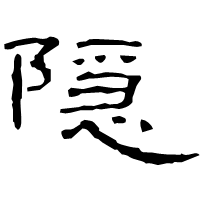
\includegraphics[width=\textwidth]{隸書/隱2}
		\caption{\content{〈曹全碑〉}{《曹全碑》}}
		\label{figure:《曹全碑》「隱」}
	\end{subcaptionblock}
	\caption{\content{「隱」字的早期写法}{“隐”字的早期写法}}
	\label{figure:「隱」字的早期寫法}
\end{figure}
\begin{wrapfigure}{O}{.2\textwidth}
	\centering
	\vspace{-2ex}
	\begin{tikzpicture}
		\begin{scope}
			\clip(0,0)rectangle(2.6,11.7);
			\node[inner sep=0pt]at(.5,6){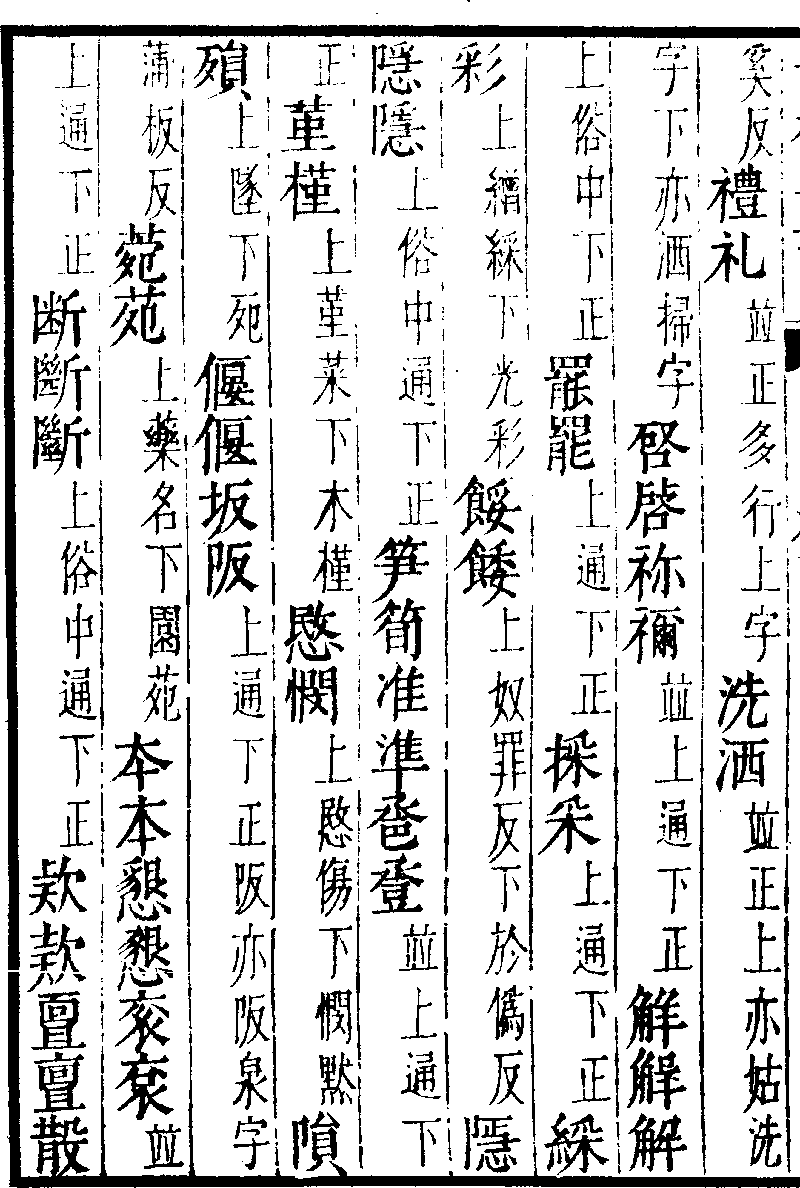
\includegraphics[height=12cm]{干祿字書-隱隠.png}};
		\end{scope}
		\draw[red](1.1,.1)rectangle(1.8,.8);
		\draw[red](.18,10.38)rectangle(.82,11.62);
	\end{tikzpicture}
	\caption{\content{《干祿字書》中的「隱」}{《干禄字书》中的“隐”}}
	\label{figure:《干祿字書》中的「隱」}
\end{wrapfigure}
\content{今天我們能看到的最早的「隱」字只有戰國的秦文字,而秦文字中已經有不同的寫法了,所以我們並不知道原始的「隱」字到底有沒有「工」。《說文》把有「工」的「隱」字定為正體,但當時的人們已經普遍使用「隠」字了,即便在很莊重的碑文上也是如此(\cref*{figure:《曹全碑》「隱」})。}{今天我们能看到的最早的“隐”字只有战国的秦文字,而秦文字中已经有不同的写法了,所以我们并不知道原始的“隐”字到底有没有“工”。《说文》把有“工”的“隱”字定为正体,但当时的人们已经普遍使用“隐”字了,即便在很庄重的碑文上也是如此(\cref*{figure:《曹全碑》「隱」})。}\par
\content{唐朝顏元孫編撰《干祿字書》時也注意到了這類現象,因此他把書中所收之字分為三類:}{唐朝颜元孙编撰《干禄字书》时也注意到了这类现象,因此他把书中所收之字分为三类:}
\begin{description}
	\item[\content{俗體}{俗体}] \content{俗體字是後起的,寫法比較簡單,可以用於民間通俗文書和日常生活當中。}{俗体字是后起的,写法比较简单,可以用于民间通俗文书和日常生活当中。}
	\item[\content{通體}{通体}] \content{通體字的寫法一般也比較簡單。它和俗體字的區別在於,俗體字出現得很晚,可能是本朝才有的;而通體字是很早以前就有的。這類文字可以用於公文等場合。}{通体字的写法一般也比较简单。它和俗体字的区别在于,俗体字出现得很晚,可能是本朝才有的;而通体字是很早以前就有的。这类文字可以用于公文等场合。}
	\item[\content{正體}{正体}] \content{正體字不僅歷史久遠,而且要見於《說文》等字典或經書、典籍之中。這種字可以用於著作、科舉\footnote{又附注說:「進士考試理,宜必遵正體,明經對策,貴合經注,本又碑書,多作八分,任別詢舊則。」可以猜想,當時的科舉考試是要求寫正體字的。如果不慎寫了通體或俗體,可能要被當作錯別字。}、碑碣等非常莊重的場合。}{正体字不仅历史久远,而且要见于《说文》等字典或经书、典籍之中。这种字可以用于著作、科举\footnote{又附注说:“进士考试理,宜必遵正体,明经对策,贵合经注,本又碑书、多作八分、任别询旧则。”可以猜想,当时的科举考试是要求写正体字的。如果不慎写了通体或俗体,可能要被当作错别字。}、碑碣等非常庄重的场合。}
\end{description}\par
\content{說回「隱」字的問題。《干祿字書》收錄了此字的三種寫法,其中的「\shiftbaseline{𨼆}」是當時的俗體,而「隠」和「隱」分別是通體和正體。《干祿字書》雖把「隱」當作正體,但也承認同樣由來已久的「隠」字才是更流行的寫法。}{说回“隐”字的问题。《干禄字书》收录了此字的三种写法,其中的“\shiftbaseline{𨼆}”是当时的俗体,而“隠”和“隱”分别是通体和正体。《干禄字书》虽然把“隱”当作正体,但也承认同样由来已久的“隠”字才是更流行的写法。}\par
\content{前面我們講不同字體並行的情況,那還只是對於「篆書」「隸書」「楷書」這一層次(書體)的介紹;然而,同樣是楷書,一個字仍可以有兩種乃至更多種寫法(字形)。我們稱這些字叫做「異體字」。「隱」與「隠」便是這樣的一對異體字。後來中國大陸進行了一系列漢字簡化運動,「隠」的異寫「隐」便成了大陸的正字;而港台仍用「隱」字,遂有了「簡體」與「繁體」的區別。其實「繁簡」本質上都是異體字關係。}{前面我们讲不同字体并行的情况,那还只是对于“篆书”“隶书”“楷书”这一层次(书体)的介绍;然而,同样是楷书,一个字仍可以有两种乃至更多种写法(字形)。我们称这些字叫做“异体字”。“隱”与“隠”便是这样的一对异体字。后来中国大陆进行了一系列汉字简化运动,“隠”的异写“隐”便成了大陆的正字;而港台仍用“隱”字,遂有了“简体”与“繁体”的区别。其实“繁简”本质上都是异体字关系。}\par
\content{還有一類異體情況是不完全的異體,即:在特定場合下,某個字既可以這樣寫又可以那樣寫;但在其它場合下就不行了。就以「記錄」「𨥈錄」來說,無論《國語辭典》還是《現代漢語詞典》都認為這兩種寫法相同,因此在表達「記錄」的含義時,「記」「紀」二字便是異體。但放在別的詞中則未必,「記憶」不能寫作「紀憶」,「紀年」不能寫作「記年」,這也是兩岸詞典公認的。}{还有一类异体情况是不完全的异体,即:在特定场合下,某个字既可以这样写又可以那样写;但在其它场合下就不行了。就以“记录”“纪录”来说,无论《现代汉语词典》还是《国语辞典》都认为这两种写法相同,因此在表达“记录”的含义时,“记”“纪”二字便是异体。但放在别的词中则未必,“记忆”不能写作“纪忆”,“纪年”不能写作“记年”,这也是两岸词典公认的。}\par
\subsubsection{\content{訛變}{讹变}}
\begin{boxquote}{\content{《示兒編·卷二十二》}{《示儿编·卷二十二》}}
	\content{久矣,倍\footnotemark 書字體,分毫㸃劃訛失,後學相承,遂成即真。}{久矣,倍\footnotemark 书字体,分毫点划讹失,后学相承,遂成即真。}
\end{boxquote}\footnotetext{\content{《四庫全書》本中為「倍」字,但應是「俗」字才合理。}{《四库全书》本中为“倍”字,但应是“俗”字才合理。}}
\content{我們曾經討論過「肝膽股肱胃腎」的偏旁本是「肉」不是「月」,只是它們在楷書中合流為「月」了。這裡還有另一個字例:「朝」。}{我们曾经讨论过“肝胆股肱胃肾”的偏旁本是“肉”不是“月”,只是它们在楷书中合流为“月”了。这里还有另一个字例:“朝”。我们看《说文》中的小篆(\cref*{figure:《說文》朝}),“朝”字从的是“舟”而不是“月”。}\par
\begin{figure}[H]
	\centering
	\begin{subcaptionblock}{.15\textwidth}
		\centering
		\includegraphics[width=\textwidth]{小篆/朝}
		\caption{\content{《說文》}{《说文》}}
		\label{figure:《說文》朝}
	\end{subcaptionblock}
	\begin{subcaptionblock}{.15\textwidth}
		\centering
		\includegraphics[width=\textwidth]{戰國/秦/朝}
		\caption{\content{戰國秦}{战国秦}}
	\end{subcaptionblock}
	\begin{subcaptionblock}{.15\textwidth}
		\centering
		\includegraphics[width=\textwidth]{戰國/晉/朝}
		\caption{\content{戰國晉}{战国晋}}
	\end{subcaptionblock}
	\begin{subcaptionblock}{.15\textwidth}
		\centering
		\includegraphics[width=\textwidth]{戰國/楚/朝}
		\caption{\content{戰國楚}{战国楚}}
	\end{subcaptionblock}
	\caption{\content{「朝」的中期寫法}{“朝”的中期写法}}
	\label{figure:「朝」的中期寫法}
\end{figure}
\content{我們看《說文》中的小篆(\cref*{figure:《說文》朝})字形,「朝」本應從「倝」,「舟」聲\footnote{按一般情況下我們對文字的理解方式,「\shiftbaseline{𦩻}」字是左右結構的。但若是分析它的形旁聲旁,則必須分成「倝」和「舟」來看待,即聲旁只佔一角。}。再看戰國文字,秦、晉文字中的「朝」都是「舟」旁;楚文字的偏旁似「舟」又似「月」,但綜合各個楚字形來看,此處應當是「舟」。}{我们看《说文》中的小篆(\cref*{figure:《說文》朝})字形,“朝”本应从“倝”,“舟”声\footnote{按一般情况下我们对文字的理解方式,“\shiftbaseline{𦩻}”字是左右结构的。但若是分析它的形旁声旁,则必须分成“倝”和“舟”来看待,即声旁只占一角。}。再看战国文字,秦、晋文字中的“朝”都是“舟”旁,楚文字的偏旁似“舟”又似“月”,但综合各个楚字形来看,此处应当是“舟”。}\par
\content{這說明,早在戰國時期,很多地方,包括後來成為正統的秦,都在用「\shiftbaseline{𰰎}」或者是它的異體字「\shiftbaseline{𦩻}」。而從隸書開始,「朝」就從「月」不從「舟」了。根據以上所述,筆者作出如下的假說:原本戰國時期的各國正體都作「\shiftbaseline{𦩻}」;各國俗體都不約而同把「𠂉」簡省掉而作「\shiftbaseline{𰰎}」;小篆字形依據秦國正體,作「\shiftbaseline{𦩻}」,這也正是《說文》中的字形;而在隸書形成的過程中「舟」旁簡化為「月」,於是就有了我們今天看到的「朝」字。}{这说明,早在战国时期,很多地方,包括后来成为正统的秦,都在用“\shiftbaseline{𰰎}”或者是它的异体字“\shiftbaseline{𦩻}”。而从隶书开始,“朝”就从“月”不从“舟”了。根据以上所述,笔者作出如下的假说:原本战国时期的各国正体都作“\shiftbaseline{𦩻}”;各国俗体都不约而同把“𠂉”简省掉而作“\shiftbaseline{𰰎}”;小篆字形依据秦国正体,作“\shiftbaseline{𦩻}”,这也正是《说文》中的字形;而在隶书形成的过程中“舟”旁简化为“月”,于是就有了我们今天看到的“朝”字。}\par
\begin{figure}[H]
	\centering
	\begin{subcaptionblock}{.2\textwidth}
		\centering
		\includegraphics[width=.7\textwidth]{甲骨文/朝}
		\caption{\content{甲骨文}{甲骨文}}
	\end{subcaptionblock}
	\begin{subcaptionblock}{.2\textwidth}
		\centering
		\includegraphics[width=.7\textwidth]{金文/朝}
		\caption{\content{西周早期金文}{西周早期金文}}
	\end{subcaptionblock}
	\begin{subcaptionblock}{.2\textwidth}
		\centering
		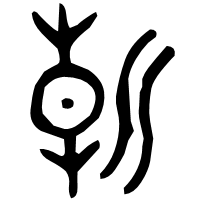
\includegraphics[width=.7\textwidth]{金文/朝1}
		\caption{\content{西周晚期金文}{西周晚期金文}}
	\end{subcaptionblock}
	\caption{\content{「朝」的早期寫法}{“朝”的早期写法}}
	\label{figure:「朝」的早期寫法}
\end{figure}
\content{但這就是真相嗎?未必。我們再看甲骨文和金文中的「朝」字(\cref*{figure:「朝」的早期寫法}),甲骨文中「朝」字就是從「月」的,是「月落日出」的表意字;而西周金文則從「川」或從「巜」。從「川」的西周金文「\includecharacter{金文/朝}」與從「舟」的戰國晉文字「\includecharacter{戰國/晉/朝}」十分相像,一旦傳抄文字過程中把前者抄成了後者的樣子,那就自然會使人誤以為「朝」字是從「舟」了——何況「朝」與「舟」古音相近,當時的人看到易混的偏旁「川」與「舟」時,自然更容易想到音近的「舟」。}{但这就是真相吗?未必。我们再看甲骨文和金文中的“朝”字(\cref*{figure:「朝」的早期寫法}),甲骨文中“朝”字就是从“月”的,是“月落日出”的表意字;而西周金文则从“川”或从“巜”。从“川”的西周金文“\includecharacter{金文/朝}”与从“舟”的战国晋文字“\includecharacter{戰國/晉/朝}」十分相像,一旦传抄文字过程中把前者抄成了后者的样子,那就自然会使人误以为“朝”字是从“舟”了——何况“朝”与“舟”古音相近,当时的人看到易混的偏旁“川”与“舟”时,自然更容易想到音近的“舟”。}\par
\content{總之,從「川」的「朝」字就在這些因素的作用下,被越來越多的人誤以為是從「舟」,最後「\shiftbaseline{𰰎}」甚至取代了原來的寫法而成為主流,這就是一個\textbf{訛變}的過程\footnote{按李學勤《字源》的說法(611頁),《說文》「\shiftbaseline{𦩻}」的形旁「倝」也是訛變而成的,本應作「\includecharacter[trim={0 0 75 0},clip]{戰國/晉/朝}」。不過沒有解釋原因。}。}{总之,从“川”的“朝”字就在这些因素的共同作用下,被越来越多的人误以为是从“舟”,最后“\shiftbaseline{𰰎}”甚至取代的原来的写法而成为主流,这就是一个\textbf{讹变}的过程\footnote{按李学勤《字源》的说法(611页),《说文》“\shiftbaseline{𦩻}”的 形旁“倝”也是讹变而成的,本应作“\includecharacter[trim={0 0 75 0},clip]{戰國/晉/朝}」。不过没有解释原因。}。}\par
\subsection{\content{漢字簡化運動}{汉字简化运动}}\label{subsection:漢字簡化運動}
\begin{wrapfigure}{O}{.4\textwidth}
	\centering
	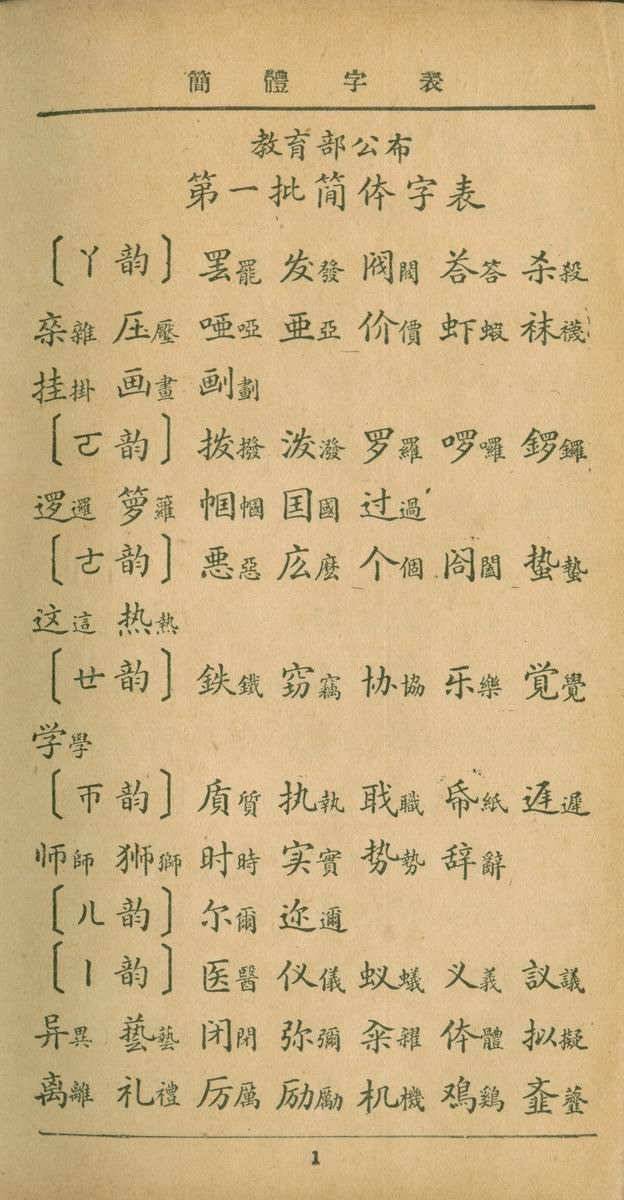
\includegraphics[width=.4\textwidth]{民國二十四年第一批簡體字表.jpg}
	\caption{\content{最早的官方簡化字嘗試}{最早的官方简化字尝试}}
	\label{figure:最早的官方簡化字嘗試}
\end{wrapfigure}
\content{中華人民共和國成立後,曾進行過兩輪漢字簡化運動。其中第一次簡化做得很成功,基本奠定了如今中國大陸使用的簡體字之標準;但第二次卻做得很失敗,以致九年後國務院收回成命,廢除了這些字。}{中华人民共和国成立后,曾进行过两轮汉字简化运动。其中第一次简化做得很成功,基本奠定了如今中国大陆使用的简体字之标准;但第二次却做得很失败,以致九年后国务院收回成命,废除了这些字。}\par
\subsubsection{\content{背景}{背景}}
\content{\cref*{figure:最早的官方簡化字嘗試}是某次政府推動漢字簡化時頒布的文件,讀者不妨猜猜,它是在什麼時期頒布的?}{\cref*{figure:最早的官方簡化字嘗試}是某次政詂推动汉字简化时颁布的文件,读者不妨猜猜,它是在什么时期颁布的?}\par
\content{或許讀者會猜測,這是1956年第一次漢字簡化運動時的文件。其實不然,這是民國二十四年(1935)嘗試推廣簡體字期間,由中華民國教育部頒布的簡體字表,共計324字。這次試推廣簡體字遭遇了很多人的反對,於是被擱置起來,暫緩實行。然而這一擱置就再也沒有實行。}{或许读者会猜测,这是1956起第一次汉字简化运动时的文件。其实不然,这是民国二十四年(1935)尝试推广简体字期间,由中华民国教育部所颁布的简体字表,共计324字。这次试推广简体字遭遇了很多人的反对,于是被搁置起来,暂缓实行。然而这一搁置就再也没有实行。}\par
\content{我們看圖中的很多「簡體字」,有不少都與現在通行的簡體字一致,比如「價」簡作「价」,「個」簡作「个」,「時」簡作「时」,「醫」簡作「医」等。當然也有一些不一致的,如「職」簡作「聀」不作「职」,「亞」簡作「亜」不作「亚」\footnote{另外,第一批簡體字表沒有做多少偏旁類推簡化,比如「質」只簡作「貭」,其「貝」旁沒有簡化為「贝」。其實這些偏旁類推簡化也是在計劃之中的,但不在第一批之列,因為每個偏旁都牽扯到很多的字,一旦做類推簡化,就需要重製大量鉛字,費時費力,反而不便於簡體字的推廣。}。總而言之,現今的簡化字不是共和國的獨創。}{我们看图中的很多“简体字”,有不少都与现在通行的简体字一致,比如“價”简体“价”,“個”简作“个”,“時”简作“时”,“醫”简作“医”等。当然也有一些不一致的,如“職”简体“聀”不作“职”,“亞”简作“亜”不作“亚”\footnote{另外,第一批简体字表没有做多少偏旁类推简化,比如“質”只简作“貭”,其“貝”旁没有简化为“贝”。其实这些偏旁类推简化也是在计划之中的,但不在第一批之列,因为每个偏旁都牵扯到很多的字,一旦做类推简化,就需要重制大量铅字,费时费力,反而不便于简体字的推广。}。总而言之,现今的简化字不是共和国的独创。}\par
\content{1935年的「簡體字」也並非民國的獨創,許多字形其實早已存在,比如在\cref{figure:「隱」字的早期寫法}中我們就能看到秦朝隸書中的「隐」(隱)字形。民國十九年(1930),史語所曾出版過一本《宋元以來俗字譜》,收䤸了由宋至清的12部古刊本\footnote{包括:宋刊本《古列女傳》《大唐三藏取經詩話》、元鈔本《京本通俗小說》、元刊本《古今雜劇三十種》《全相三國志平話》《朝野新聲太平樂府》、明刊本《嬌紅記》《薛仁貴跨海征東白袍記》《岳飛破虜東牕記》、清刊本《目蓮記彈詞》《金瓶梅奇書前後部》《嶺南逸史》。}中出現的各種俗字。筆者簡單統計了一些俗字,列於\cref*{table:《宋元以來俗字譜》12古刊本中出現俗字的情況}中。}{1935年的“简体字”也并非民国的独创,许多字形其实早已存在,比如在\cref{figure:「隱」字的早期寫法}中我们就能看到秦朝隶书中的“隐”字形。民国十九年(1930),史语所曾出版过一本《宋元以来俗字谱》,收录了由宋至清的12部古刊本\footnote{包括:宋刊本《古列女传》《大唐三藏取经诗话》、元钞本《京本通俗小说》、元刊本《古今杂剧三十种》《全相三国志平话》《朝野新声太平乐府》、明刊本《娇红记》《薛仁贵跨海征东白袍记》《岳飞破虏东窗记》、清刊本《目莲记弹词》《金瓶梅奇书前后部》《岭南逸史》。}中出现的各种俗字。笔者简单统计了一些俗字,列于\cref*{table:《宋元以來俗字譜》12古刊本中出現俗字的情況}中。}\par
\begin{table}[H]
	\centering
	\caption{\content{《宋元以來俗字譜》12古刊本中出現俗字的情況}{《宋元以来俗字谱》12古刊本中出现俗字的情况}}
	\label{table:《宋元以來俗字譜》12古刊本中出現俗字的情況}
	\begin{NiceTabular}{*{8}{c}}[hlines]
	\CodeBefore
		\rowcolor{lightgray}{1}
		\columncolor{lightgray}{1,5}
	\Body
		\toprule
		俗字 & \content{出現次數}{出现次数} & \content{正體字}{繁体字} & \content{簡體字}{简体字} & 俗字 & \content{出現次數}{出现次数} & \content{正體字}{繁体字} & \content{簡體字}{简体字} \\\midrule[.6pt]
		阳 & 5 & 陽 & 阳 & 医 & 6 & 醫 & 医 \\
		义 & 6 & 義 & 义 & 时 & 7 & 時 & 时 \\
		罗 & 7 & 羅 & 罗 & 云 & 9 & 雲 & 云 \\
		鉄 & 9 & 鐵 & 铁 & 囯 & 10 & 國 & 国 \\
		灵 & 10 & 靈 & 灵 & 个 & 11 & 個 & 个 \\
		声 & 12 & 聲 & 声 & 宝 & 12 & 寶 & 宝 \\\bottomrule
	\end{NiceTabular}
\end{table}
\content{宋朝以來,通俗讀物就已經隨著印刷術的興盛而普及開來,所以當時的通俗讀物可以反映當地民間的漢字使用情況。我們今天熟知的很多「簡體字」,其實早在那時就已在民間廣泛使用了。只不過,直至1935年,這些簡俗字都未曾獲得過官方認可的合法地位,只是作為「異體字」存在。而1935年的簡化字也不過是曇花一現,並未真正推廣開來。}{宋朝以来,通俗读物就已经随着印刷术的兴盛而普及开来,所以当时的通俗读物可以反映当地民间的汉字使用情况。我们今天熟知的很多“简体字”,其实早在那时就已在民间广泛使用了。只不过,直至1935年,这些简俗字都未曾获得过官方认可以合法地位,只是作为“异体字”存在。而1935年的简化字也不过是昙花一现,并未真正推广开来。}\par
\subsubsection{\content{行書、草書楷化}{行書、草书楷化}}
\begin{figure}[H]
	\centering
	\captionbox{\content{「時」的草書}{“時/时”的草书}\label{figure:草书-時}}{
		\centering
		\begin{subfigure}[t]{.2\textwidth}
			\centering
			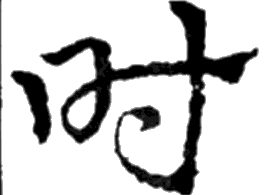
\includegraphics[trim={5 0 0 0},clip,height=2.5cm]{今草/時-皇象}
			\caption{\content{皇象(三國吳)}{皇象(三国吴)}}
		\end{subfigure}
		\begin{subfigure}[t]{.2\textwidth}
			\centering
			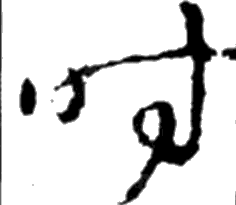
\includegraphics[trim={5 0 0 0},clip,height=2.5cm]{今草/時-王羲之}
			\caption{\content{王羲之(東晉)}{王羲之(东晋)}}
		\end{subfigure}
	}
	\captionbox{\content{褚遂良書法「馬」}{褚遂良书法“馬/马”}\label{figure:褚遂良書法「馬」}}{
		\centering
		\begin{subfigure}[t]{.2\textwidth}
			\centering
			\includegraphics[trim={7 4 0 0},clip,height=2.5cm]{楷書/馬-褚遂良}
			\caption{\content{楷書}{楷书}}
		\end{subfigure}
		\hspace{-.5cm}
		\begin{subfigure}[t]{.2\textwidth}
			\centering
			\includegraphics[trim={5 0 0 0},clip,height=2.5cm]{行書/馬-褚遂良}
			\caption{\content{行書}{行书}}
		\end{subfigure}
	}
\end{figure}
\content{作為印刷體的明體是脫胎於楷書的,而作為書法體的楷書本來並沒有「时」這個字形。那麼明體中的「时」字形是哪裡來的呢?答案在草書中。}{作为印刷体的宋体是脱胎于楷书的,而作为书法体的楷书本来并没有“时”这个字形。那么宋体中的“时”字形是哪里来的呢?答案在草书中。}\par
\content{早在魏晉時期的草書中我們就可以看到「时」這樣的字形(\cref*{figure:草书-時})。後世的「時」字草書一般也是寫作如此。這種寫法是獨屬於草書的,楷書和行書中並不存在這樣一個左「日」右「寸」的字形。}{早在魏晋时期的草书中我们就可以看到“时”这样的字形(\cref*{figure:草书-時})。后世的“时”字草书一般也是写作如此。这种写法是独属于草书的,楷书和行书中并不存在这样一个左“日”右“寸”的字形。}\par
\content{但是,民間俗寫才不會在乎哪個書體,人們只是傾向於那些寫起來方便、簡單的字形。而在這方面,行書、草書的寫法顯然要比楷書更有優勢(狂草也簡單,但是看不懂)。於是人們根據行書或草書的結構,用楷書的筆法寫出一個新字形來,這就是\textbf{行書楷化}或\textbf{草書楷化}。}{但是,民间俗写才不会在乎哪个书体,人们只是倾向于那些写起来方便,简单的字形。而在这方面,行书、草书的写法显然要比楷书更有优势(狂草也简单,但是看不懂)。于是人们根据行书或草书的结构,用楷书的笔法写出一个新字形来,这就是\textbf{行书楷化}或\textbf{草书楷化}。}\par
\content{一個典型的行書楷化示例是「馬」字的四點化一橫。我們看唐朝褚遂良的楷書「馬」和行書「\shiftbaseline{𫠉}」,就能明顯比較出來(\cref*{figure:褚遂良書法「馬」})。楷書「馬」一般是寫作四點的,行書寫得快了,連筆起來就成一橫了。簡化字「马」的一橫自然是取了行書的寫法再楷化得到的。}{一个典型的行书楷化示例是“马”字的四点化一横。我们看唐朝褚遂良的楷书“馬”和行书“\shiftbaseline{𫠉}”,就能明显比较出来(\cref*{figure:褚遂良書法「馬」})。楷书“馬”一般是写作四点的,行书写得快了,连笔起来就成一横了。简化字“马”的一横自然是取了行书的写法再楷化得到的。}\par
% \subsection{\content{二簡字}{二简字}}
% \begin{boxquote}{\content{裘錫圭《文字學概要》}{裘锡圭《文字学概要》}}
% 	\content{為了把象形的古文字改造成隶、楷而破壞一部分字的結構,是迫不得已的,也是值得的。在楷書早已成熟的情況下,仅仅為了減少筆畫而去破壞某些字的結構,把它們變成記號字,這樣做究竟是不是必要,是不是值得,就大可懷疑了。}{为了把象形的古文字改造成隶、楷而破坏一部分字的结构,是迫不得已的,也是值得的。在楷书早已成熟的情况下,仅仅为了减少笔画而去破坏某些字的结构,把它们变成记号字,这样做究竟是不是必要,是不是值得,就大可怀疑了。}
% \end{boxquote}
